\documentclass[12pt,a4paper,titlepage]{article}
\usepackage{main-styles}
\usepackage{thesis-constants}

\usepackage{pdfpages}
\usepackage{tikz}
\usepackage{times}

\usetikzlibrary{matrix}

% the document should be compiled with pdfLaTex

\begin{document}

\phantomsection

%##############################################################################

\begin{titlepage}

    \newcommand{\HRule}{\rule{\linewidth}{0.5mm}}

    \UniversityHeader
    \center

    \vspace{2cm}
    \textbf{
        \hfill Admis la susținere\\
        \hfill Șef de departament:\\
        \hfill Fiodorov I. dr., conf.univ.\\
    }

    \vspace{0.4cm}
    \hfill "\rule{0.75cm}{0.2mm}" \ \rule{3cm}{0.2mm} \the\year
    \vspace{2cm}



    \begin{center}
        \Large \textbf{\ThesisTitle}\\
        \vspace{0.6cm}
        Proiect de licență
    \end{center}
    \vspace{1cm}


    \hfill Student: \rule{4.5cm}{0.2mm} \MyNameFull\\
    \vspace{0.2cm}

    \hfill Coordonator: \rule{4.4cm}{0.2mm} \CoordonatorFull\\
    \vspace{0.2cm}

    \hfill Consultant: \rule{4cm}{0.2mm} Catruc Mariana, lect.univ.\\
    \vspace{0.2cm}

    \hfill Consultant: \rule{4cm}{0.2mm} Prodan-Șestacova Liubovi,\\\hfill dr., conf.univ.\\
    \vspace{0.2cm}

    \vspace{5cm}

    \vfill
    \begin{center}
        Chișinău, \the\year
    \end{center}
\end{titlepage}

\cleardoublepage

\begin{titlepage}

    \newcommand{\HRule}{\rule{\linewidth}{0.5mm}}
    
    \UniversityHeader
    \center
    
    \vspace{2cm}
    \textbf{
        \hfill Aprob\\
        \hfill șef de departament\\
        \hfill Fiodorov Ion, dr.conf.univ.\\
    }
    
    \vspace{0.4cm}
    \hfill \textbf{"\underline{30}" \ \underline{octombrie} 2019}
    \vspace{2cm}

    
    
    \begin{center}
    \large \textbf{CAIET DE SARCINI} \\
    \vspace{0.2cm}
    \large \textbf{pentru proiectul de licență} \\
    \vspace{0.2cm}
    \large \MyName
    
    \end{center}
    
    \begin{enumerate}
    \item[1.]  \textbf{Tema proiectului de licență}: \ThesisTitle \\\ \textbf{confirmată prin hotărârea Consiliului facultății nr. \underline{1}} din \textit{"\underline{30}" \ \underline{octombrie} 2019}
    
    \item[2.]  \textbf{Termenul limită de prezentare a proiectului}: \textit{14.05.2020}
    
    \item[3.]  \textbf{Date inițiale pentru elaborarea proiectului} Sarcina pentru elaborarea proiectului de diplomă
    
    \item[4.]  \textbf{Conținutul memoriului explicativ}
    
    \begin{enumerate}
        \item[] Introducere
        \item[1.]Analiza domeniului de studiu
        \item[2.]Proiectarea sistemului
        \item[3.]Realizarea sistemului
        \item[4.]Documentarea produsului realizat
        \item[5.]Argumentarea economică
        \item[] Concluzii
    \end{enumerate}

    \item[5.]  \textbf{Conținutul părții grafice a proiectului} \\Diagrama \textbf{Use Case} generală a sistemului, \textbf{Interfața Principală} a programului.
    
    \newpage
    
    \item[6.]  \textbf{Lista consultațiilor} 
    
    \begin{tabular}{ |p{3 cm}|p{4 cm}| p{3cm} |p{4cm}|  }
     \hline
     \multirow{3}{*}{} & & \multicolumn{2}{ c|}{\textbf{Confirmarea realizării activității}}  \\
    \multicolumn{1}{|c|}{\multirow{2}{*}{\textbf{Consultant}}} & \multicolumn{1}{ c|}{\multirow{2}{*}{\textbf{Capitol}}}  & \multicolumn{2}{ c|}{}\\
    \cline{3-4}
     &  & \multicolumn{1}{c|}{\begin{tabular}[c]{@{}c@{}}Semnătura\\ consultantului (data)\end{tabular}} & \multicolumn{1}{c|}{\begin{tabular}[c]{@{}c@{}}Semnătura\\ studentului (data)\end{tabular}}  \\
    \hline
    
    \begin{tabular}[c]{@{}l@{}}L. Prodan-\\Șestacova\end{tabular} & Argumentarea \newline economică  & &   \\
    \hline
     M. Catruc  &  \begin{tabular}[c]{@{}l@{}}Controlul calității, \\ standarde tehnologice\end{tabular}  & &\\
     
     \hline
    \end{tabular}
    \\
    \item[7.]  \textbf{Data înmânării caietului de sarcini}: \textit{\underline{02.09.2019}}
    
    \end{enumerate}
    
    
    \vspace{1cm}
    \textbf{
        \hfill Coordonator\\
        \hfill \CoordonatorFull\\
    }
    
    \vspace{0.4cm}
    \hfill Semnătura  \ \rule{5cm}{0.2mm}
    \vspace{0.8cm}
    
    \textbf{Sarcina a fost luată pentru a fi executată de către studentul } \MyName
    
    \vspace{0.2cm}
    \ \rule{5cm}{0.2mm} \textit{02.05.2020}
    
    \vspace{0.8cm}
    \textbf{PLAN CALENDARISTIC}
    \vspace{0.4cm}
    
    \begin{tabular}{ |p{1cm}||p{8cm}|p{5cm}|p{2cm}|  }
        \hline
        \textbf{Nr. crt.} & \textbf{Denumirea etapelor de proiectare }   &\textbf{Termenul de realizare a \newline etapelor }& \textbf{Nota}  \\

        \hline
        1 & Elaborarea sarcinii, primirea datelor pentru \newline sarcină  & 02.09.19– 30.09.19 & 10\% \\

        \hline
        2 & Analiza domeniului de studiu & 01.10.19– 30.11.19 & 20\%\\

        \hline
        3 & Proiectarea sistemului & 01.12.19 – 25.12.19 & 20\% \\

        \hline
        4 & Realizarea sistemului & 16.01.20 – 14.03.20 & 25\% \\

        \hline
        5 & Descrierea sistemului & 15.03.20– 10.04.20 & 10\% \\

        \hline
        6 & Testarea sistemului & 11.04.20– 20.04.20 & 10\% \\
        
        \hline
        7 & Finisarea proiectului & 21.04.20– 08.05.20 & 5\% \\
        
        \hline
    \end{tabular}
    
    \vspace{1cm}
    \hfill Student: \rule{4.5cm}{0.2mm} \MyName\\
    \vspace{0.2cm}
    \hfill Coordonator de proiect de licență: \rule{4.5cm}{0.2mm} \Coordonator\\
    \vspace{0.2cm}

\end{titlepage}

\cleardoublepage

\begin{center}
    \vspace{2cm}
    \fbox{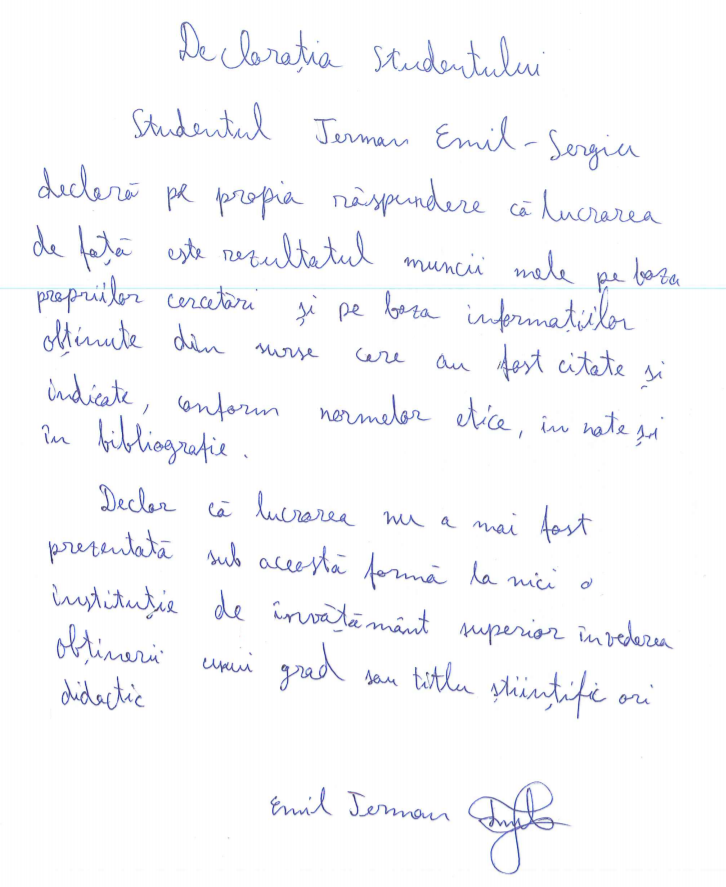
\includegraphics{declaration}}
\end{center}
\cleardoublepage

\begin{titlepage}

    \newcommand{\HRule}{\rule{\linewidth}{0.5mm}}
    
    \begin{center}
        \textbf{
            Universitatea Tehnică a Moldovei\\
            Facultatea Calculatoare, Informatică și Microelectronică\\
            Departamentul Ingineria Software și Automatică\\
            Programul de studii Tehnologii Informaționale\\
        }
    \end{center}
    \center
    
    \vspace{0.3cm}
    \begin{center}
        \large \textbf{AVIZ} \\
        Teza de licenţă \\
    \vspace{0.2cm}
    
    \end{center}
    
    \begin{flushleft}
        \textbf{Tema:} \ThesisTitle \\
        \textbf{Studentul:} \MyNameFull
        
        \begin{enumerate}[leftmargin=1.4em, itemsep=1pt, parsep=0pt]
        \item [1.] \textbf{Caracteristica tezei de licență:}  Teza a fost elaborată în conformitate cu toate cerințele și standardele în vigoare; reprezintă o analiză detaliată a implementărilor existente, depășind domeniul imediat al implementării soluției propuse și analizînd scenarii similare în alte domenii. Teza reprezintă un vestigiu coerent al lucrului intelectual efectuat de către student.
        
        \item [2.] \textbf{Estimarea rezultatelor obținute:} Rezultatele obținute sunt deja aplicabile; aplicația e bine documentată, iar codul este deloc criptic, bine organizat și elaborat cu responsabilitate.
        
        \item [3.] \textbf{Corectitudinea materialului expus:} Referințele externe au fost luate din surse respectabile, iar sinteza informației obținute în rezultatul lucrului și a evaluării surselor externe este concludentă și logică. Teza corespunde standardelor tehnice, inclusiv analiza economică a proiectului și diagramele utilizate. 
        
        \item [4.] \textbf{Calitatea materialului grafic:} Figurile prezentate în lucrarea dată descriu si analizeaza în detaliu sistemul curent. Diagramele UML corespund standartului 2.0. Materialul grafic prezentat în lucrare îşi îndeplineşte scopul de a îmbunătăţi descrierea sistemului impementat.
        
        \item [5.] \textbf{Observații și recomandări:} Această teză se face evidentă, în primul rînd, datorită caracterului practic al problemei pe care o abordează. Este recomandat de a extinde sistemul curent cu noi funcţionalităţi.
        
        \item [6.] \textbf{Caracteristica studentului și titlul conferit:} Studentul a demonstrat o asiduitate deosebită în studierea independentă a unei teme netriviale și o abordare inginerească în soluționarea problemei specificate.
        
        \textbf{Rezultatele obținute în cadrul tezei îmi permit să recomand admiterea tezei de licență d-lui \MyName spre susținere și să o apreciez cu nota maximă.}
        
        \end{enumerate}
        
        \hfill Conducătorul tezei de licență\\
        \hfill \textbf{\Coordonator}\\

    \end{flushleft}
    \vfill
\end{titlepage}
\cleardoublepage

\input{abstract.tex}
\clearpage

\input{rezumat.tex}
\clearpage

\tableofcontents
\addtocontents{toc}{\protect\thispagestyle{empty}}
\cleardoublepage

\listoffigures
\addcontentsline{toc}{section}{List of figures}
\clearpage

\lstlistoflistings
\addcontentsline{toc}{section}{Listings}
\thispagestyle{empty}
\clearpage

\phantomsection
\addcontentsline{toc}{section}{Abbreviations}
\input{abbreviations.tex}
\thispagestyle{empty}
\cleardoublepage

\phantomsection
\addcontentsline{toc}{section}{Introduction}
\input{introduction.tex}
\cleardoublepage

\section{Project analysis and System requirements}
\phantomsection

\subsection{Problem Definition}
A photographer tasked with year long time-lapse usually spends its friday checking on the time-lapses. He would usually use an application like TeamViewer or another Remote Desktop application to connect to the computer that has the cameras connected to. He would have to manually check if the desktop application is still running and if it had any failures. If he is lucky enough, he might have written a script that opens the application on startup and program the mouse to start the time-lapse again from the last index, only if no additional pop-ups appear in the meantime. On the other hand, if the time-lapse is very expensive, say it's a very expensive experiment that requires a few weeks time-lapse, then the photographer would have for each camera an open remote desktop to see if it is still working.

It becomes exponentially difficult to automate this entire process for different models of cameras. In big enterprises usually the photographer is given a set o company owned cameras, which often come from different brands: Canon, Nikon, Sony, Pentax, Olympus, etc. Each brand usually comes with its own specific software, so it becomes next to impossible to write an all purpose reliable script to automate a time-lapse composed of multiple different cameras.

Taking continuous high quality time-lapses is one of the most challenging work that can be done by a photographer.

\subsection{Project Analysis}
DSLR Camera Controller is a tool which aims to provide easy access and management of cameras, supporting a wide range of models, through a web browser. The main features are:
\begin{enumerate}
    \item Live preview;
    \item Take a picture;
    \item Camera configuration;
    \item Failure strategy:
    \begin{itemize}
        \item Send email;
        \item Hard reset;
        \item Reboot system after N failures;
    \end{itemize}
    \item Time-lapse scheduling;
    \item File transfer;
    \item Photo name patterns:
    \begin{itemize}
        \item Time (timestamp, hour, minute, day, year, etc);
        \item Capture index;
        \item Camera serial number;
        \item Camera name;
        \item Time-lapse name;
    \end{itemize}
\end{enumerate}

\subsubsection{Failure strategy}
A camera can fail because of a variety of reasons. Some models, automatically go to into sleep mode when the connected computer does not send any commands for an hour. This happens very often, as some time-lapses usually happen during the working days. Another common case is when the local workers simply unplug the device, or trip on the cable. Other times the power is simply cut off for a brief period of time, causing some confusion on some models. So choosing a failure strategy is very important to reduce the time the user has to spend on the app.

One of the main problems the photographers have with time-lapses is that it can fail silently, meaning that it can encounter a failure and stop working, without the notice of the user. This is a critical problem for long time-lapses, because in most cases, it is unacceptable to have gaps in the time-lapse, especially gaps for weeks or months. To allow the user to be notified of any failures, he can enable failure email notifications, which will send notifications to the specified emails with data about the failure.

Getting failure emails every minute may not be quite the best solution when the user simply has to re-plug the camera. Re-plugging the camera solves the problem most of the time, so it is worth investing in a tool that does just that. Ykush is a device that allows automatic re-plugging of USB devices, therefore the application supports this option as well, in case the user has one connected. Enabling hard resetting on failure, will trigger any Ykush boards but it will also try to reconnect to the cameras internally, which for some cameras it works too.

Having a general solution that will work almost for sure for all models is very hard to come by, and even harder to keep it up to date, so in case the user does not want to purchase any extra external devices, a system reboot might be satisfactory The user can configure an automatic system reboot in case the camera fails N times in a row.

\subsubsection{Time-lapse scheduling}
It is not an easy task to create a tool that will combine all kinds of scheduling the user can come up with. So a solution to this problem is to use the Cron utility.

Cron is a time-based software utility for job scheduling in Unix like systems. It allows to express schedules to run periodically at fixed times, dates or intervals. While it will allow the user to express almost any kind of schedule he wants, he will have to learn a bit about cron scheduling, but attaching some of the most common cases to help them out should solve this problem.

\subsubsection{Photo name patterns}
File name collision might be a nightmare in some applications. In one case, the person in charge of time-lapses had to use a software, that did not support naming patterns, so the files were coming out appended with an index. This only worked until  the application was closed. So he had to manually check what was the last index so that the files won't overwrite. In another case, he forgot to change the index, so a 2 week time-lapse was simply overwritten without his notice.

Allowing the user to create a custom file pattern is important for making sure that nothing gets erased. It would also allow the user to easily create batch time-lapses every month/week.

\subsubsection{Web Client}
The biggest problem with the existing applications is that it only offers a desktop version. Meaning, that the only way to remotely control a camera from home, is to use an application like Remote Desktop to control the whole computer. This is still a satisfactory solution. But for some cases it becomes absolutely impossible, as it requires a relatively high bandwidth for relatively little data. For some experiments, in tunnels with no internet coverage modems are a pretty viable solution. But using remote desktop every week through modems that are barely able to connect to the internet is not the most realistic solution. Therefore, a web client would probably be the best way to approach this problem. The client side will represent a web application, a minimalist layer used for communication with the user. The web infrastructure makes the application easy to access. The requirement to run the client side application is to have a modern web browser, for instance Google Chrome, Firefox etc.

\subsection{Theoretical Analysis}
Considering the complexity of the application, a right amount of research is required in order to construct a workable tool. The final product represents a workable application focused mainly on a small niche for remote long term time-lapses. Further will follow a more detailed description of various aspects of the platform, regarding the technologies best suited for building the application, the concepts behind different tools used in the application and means for solving specific problems.

\subsection{Web Services}
Building complex systems is not a simple task and usually it consist of smaller logical parts that communicates trough interfaces. To allow further extension of the product, it would be wise to expose an API so that other applications can use it. It is easier to understand how a system works once it is decoupled in multiple independent modules. A small logical unit can be understood faster and better and once it breaks down it is easier to fix it. In the end the point is that the applications should be able to communicate efficiently over the web. Various software are built in different programming languages, are running on diverse operating systems, hence a transparent communication model is needed and at the same time is language agnostic. That is how the web services protocols came to existence. During the time they have evolved into a set of communication standards that offered developers the opportunity to construct decoupled systems.

In order to define the standards, a set of rules are needed to be defined, such as:
\begin{itemize}
    \item How can a software perform a request to another system;
    \item What is the set of parameters that should be set in the request;
    \item What should be format of the request looks like;
    \item What are the logical parts that the request consists of;
    \item How should the response be represented;
    \item How should the errors be described.
\end{itemize}

As a result, on the market usually persist two main approaches of constructing web services, SOAP and REST. Each approach have their strong points and weaknesses and both heavily relies on HTTP protocol, in case of SOAP it also supports other transport protocols.

\textbf{SOAP} is a messaging protocol that have the entire architecture wrapped around XML data representation. In a nutshell, it is a method of communication between two applications. An example of SOAP communication is represented in figure \mbox{\ref{soap}} The protocol specifies how exactly the HTTP headers should be encoded. A SOAP provider comes in hand with a WSDL file which represents the description of the web service. Things like the possible parameters and their formats, the structure of the message, what is the response format, how it can be correctly accessed. The communication via SOAP protocol is also done using XML formatted files. The structure of the the request and response is documented in the WSDL file and it is validated with the help of XSD schema.

\begin{figure}[!ht]
\centering
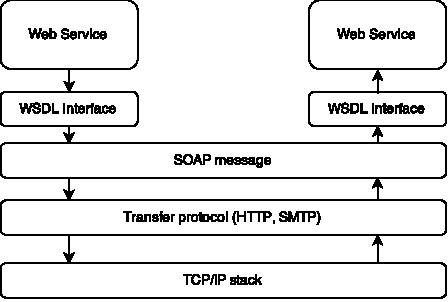
\includegraphics[width=11.5cm]{1_soap}
\caption{An example of SOAP communication}\label{soap}
\end{figure}


SOAP represents the next evolving stage between computer communication at he application layer. It was able to replace RPC technologies such as DCOM, CORBA, Java RMI. This reinstatement was highly needed because RPC technologies were brining a complex coupling to the programming language, which is definitely not a good thing. On the other hand the SOAP calls are much slower comparing to native RPC applications. There tends to be firewall latency due to the fact that the firewall is analyzing the HTTP transport. SOAP calls are much more likely to get through firewall servers, since HTTP is typically Port 80 compliant, where other calls may be blocked for security reasons. Since HTTP requests are usually allowed through firewalls, programs using SOAP to communicate can be sure that the program can communicate with programs anywhere. SOAP focuses on exposing pieces of application logic (not data) as services, platform operations. It aims for accessing named operations, each implement some business logic through different interfaces. An advantage offered by SOAP is the WS-Security which adds some enterprise security features. Supports identity through intermediaries, not just point to point (SSL). It also provides a standard for integrity.

\textbf{REST} is a simple stateless architecture that generally runs over HTTPS/TLS protocols. The flexibility is given by assigning resources their URI. The neat part is that it heavily relies on URLs. The REST philosophy is deeply entangled with HTTP protocol implementation, for instance the HTTP verbs GET, POST, PUT, DELETE, PATCH etc, are a part of REST RFC. Although it is a set of guidelines and best practices, many might understand it in their own way. Therefore, what usually happens is that the whole application is filled only with "GET" and "POST" requests. In some cases, some may even use the "GET" endpoints for creating resources, which will only confuse the reader. So this is a double-edged sword. Hence a lot of debates and discussions are still happening even today. The good part is that it doesn't need tedious descriptor files such as WSDL in order to describe a REST application. Modern frameworks usually offer a way to automatically create documentation, such as "Swagger". REST did not only impact the web architecture but it has also affected how we think about software in general. Striving to write stateless code has forever changed our mindsets, because there were times that some would think that it is absolutely fine to have methods with side effects. REST gained a lot of popularity as being a simpler alternative to SOAP and WSDL-based web services. And the most viable example is the implementation of the entire Word Wide Web. One strong thing wielded by REST applications is that the message and response content can be delivered in any format. The most used are XML based format such as HTML, and for API platforms JSON is the most common and handy format, and it has lots of advantages against XML, such as readability, payload size, easy integrable with dynamic languages, it is data oriented.

Nowadays JSON is becoming the preferred format especially for RESTful APIs. Because of the format simplicity sometimes it gets harder to define the communication structure. Which is why JSON community is working now on an elegant format called JSON-api. It simplifies a lot of things in terms of message structure. It resembles to WSDL only it is less restrictive and more intuitive. Another alternative for structuring the message format is HATEOAS. The purpose it aims is defining application state using hypertext.

\subsubsection{Data Storage}
The whole idea of computer science is wrapped around of ways of manipulating data. From the very start engineers had issues with finding ways to store data. During the time, the hardware evolved and nowadays the disk space does not represent a problem anymore. The actual challenge is how to make interaction with data as efficiently as possible. Interaction represents means of reading, and querying data, effectively saving it on the disk, keeping it consistent and avoid data loss. What if data is related to other data types. How to  implement the relationship between the data. How to make possible for multiple users to read and write at the same time. These are the actual problems which are confronted in computer science.

The classical solution to this problem are the RDBMS approaches. It is a common choice for the storage of information in new databases used for financial records, manufacturing and logistical information, personal data, and other applications since the 1980s. Relational databases have often replaced legacy hierarchical databases and network databases because they are easier to understand and use. The relational databases rely on SQL which is a special-purpose language designed for managing data. It is used to query, insert, update and modify data. RDBMS were and still are an irreplaceable solution for managing efficiently relatively small amounts of data. The RDBMS philosophy is built around ACID principle, Atomicity, Consistency, Isolation and Durability. The combination of this four principles has granted such a big success to relational databases.

As mentioned above RDBMS is widely used for lots of applications and successfully solves problems and there hasn't been a better alternative on the market. The competition is applied to different implementations of databases, such as PosgreSQL, MySQL, OracleSQL, MsSQL, MariaDB. All of them are quite similar, and each has its strong and weak points. The actual problem appears when the Big Data started to get more an more popular. Unfortunately the classical database approach was not enough for the constantly data increase. RDBMS enforces a well defined schema, as a result it gets slower and unmanageable when the amount of data gets bigger.

What developers decided was to loosen up one of the ACID principle and create new brand of databases which have a different structure and would allow storing and working with big amounts of data. This is how the term BASE principal came to life. Basically Available, Eventually Consistent. BASE concept supports the idea of network partitioning, which means that the database will always have a response disregarding the amount of requests at the given time. The catch is what kind of response should it have in case of multiple access to the database. Two solutions were proposed. First one is that the database should always return a result even though it is not up to date. The second solutions is to inform the database user that the service is not available for now. Both solutions have their own applications. Choosing which one to use depends entirely on what it is better suited for the business. The idea of choosing the database model is also presented by CAP theorem. CAP states that when choosing a database you can choose only two of the three features. These are Consistency, Availability and network Partition tolerance. In figure \mbox{\ref{cap}} is illustrated in more details the CAP and databases categorized based on theorem.

\begin{figure}[!ht]
\centering
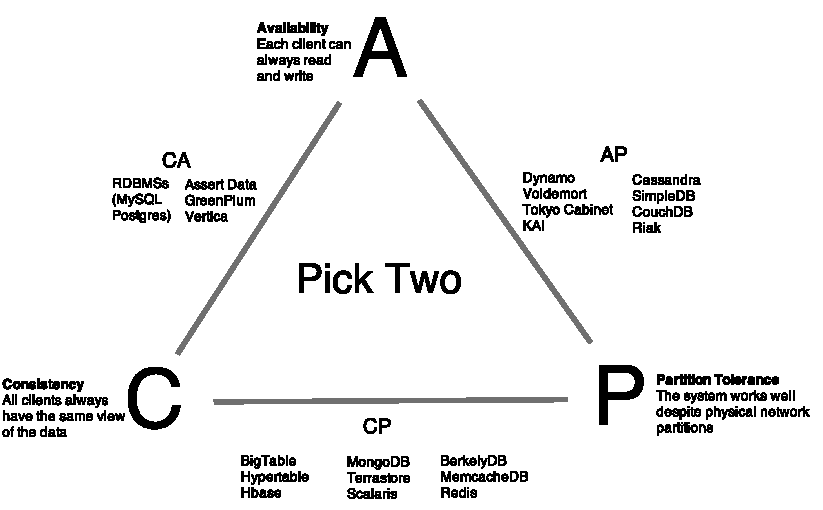
\includegraphics[width=17cm]{1_cap}
\caption{An illustration of CAP Theorem}\label{cap}
\end{figure}

Along with the implementation of conceptual new database the term NoSQL started to spread. The term came from the fact that the new databases were not using SQL for data management. In reality there are more types of conceptual database, and covering all of them under the same umbrella seems too ambiguous.
The most widely used types of databases, not considering RDBMS, are described bellow.

\textbf{Document Based Database} is a new approach of database management. It is used in usual English sense of a group of data that encodes some sort of user-readable information. This contrasts with the value in the key-value store, which is assumed to be opaque data. The basic concept that makes a database document-oriented as opposed to key-value is the idea that the documents include internal structure, or metadata, that the database engine can use to further automate the storage and provide more value.

Document databases contrast strongly with the traditional relational database (RDBMS). Relational databases are strongly typed during database creation, and store repeated data in separate tables that are defined by the programmer. In an RDBMS, every instance of data has the same format as every other, and changing that format is generally difficult. Document databases get their type information from the data itself, normally store all related information together, and allow every instance of data to be different from any other. This makes them more flexible in dealing with change and optional values, maps more easily into program objects, and often reduces database size. This makes them attractive for programming modern web applications, which are subject to continual change in place, and speed of deployment is an important issue. The current most popular implementation of such type of database is MongoDB and CouchDB.

\textbf{Column Based Database} is a database management system that stores data tables as sections of columns of data rather than as rows of data. In comparison, most relational DBMSs store data in rows. This column-oriented DBMS has advantages for data warehouses, customer relationship management systems, and library card catalogs, and other ad hoc inquiry systems where aggregates are computed over large numbers of similar data items.

It is possible to achieve some of the benefits of column-oriented and row-oriented organization with any DBMSs. Denoting one as column-oriented refers to both the ease of expression of a column-oriented structure and the focus on optimizations for column-oriented workloads. This approach is in contrast to row-oriented or row store databases and with correlation databases, which use a value-based storage structure. Such type of database implementations are BigTable, Casandra.

\textbf{Key Value Database} use the associative array (also known as a map or dictionary) as their fundamental data model. In this model, data is represented as a collection of key-value pairs, such that each possible key appears at most once in the collection. The key-value model is one of the simplest non-trivial data models, and richer data models are often implemented on top of it. The key-value model can be extended to an ordered model that maintains keys in lexicographic order. This extension is powerful, in that it can efficiently process key ranges. Example of such type of database implementations are Redis, Memcache, Voldemort.

\subsubsection{Modern Web Application}
Web applications are heavily using HTTP protocol as means of transporting data. HTTP is a stateless protocol. For every request made by a client a TCP socket is opened. The HTTP server receives a request that is handled by the application layer. When the response is sent back to the client, the TCP socket is closed and the transaction ends. The whole chain of events is repeated basically at every user interaction. The result is that a simple web application has a stateless behavior. The application layer of a web applications aims to get rid of statelessness. In 2004 the concept of web 2.0 surfaced. Javascript started to become more popular because it gave the power to animate the pages and create a more humane UX. The magic was behind the AJAX technology. The concept introduced by AJAX was making a web page run asynchronous requests and make live partially DOM changes. Developers could create web applications which did not require full page reload at while interacting with a web page. Successfully implementation of this concepts are Facebook, Gmail, Twitter etc. AJAX, JQuery and other Java Script technologies brought web applications one step closer to the desktop applications experience.

Nowadays the single page applications are becoming a hot topic. The main reason is that they are able to offer more native application like experience to the user. This is hard to do with other approaches. Supporting rich interactions with multiple components on a page means that those components have many more intermediate states. Server side rendering is hard to implement for all the intermediate states. Small view states do not map well to URLs.

Single page applications are distinguished by their ability to redraw any part of the UI without requiring a server round trip to retrieve HTML. This is achieved by separating the data from the presentation of data by having a model layer that handles data and a view layer that reads from the models. Interaction with the single page application often involves dynamic communication with the web server behind the scenes.

Here are enumerated a set of technologies that helps of building single page applications:
\begin{itemize}
    \item Ember;
    \item Angular;
    \item React;
    \item Meteor;
    \item Marionette.
\end{itemize}

Due to the fact that single page applications have a rich functionality, they also include a complex architecture. For instance in figure \mbox{\ref{ember_architecture}} is illustrated the conceptual structure of Ember framework. It is hard to wrap the head around the structure, but once there is a basic understanding of the logical layers, building applications is a joy for a developer.

\begin{figure}[!ht]
\centering
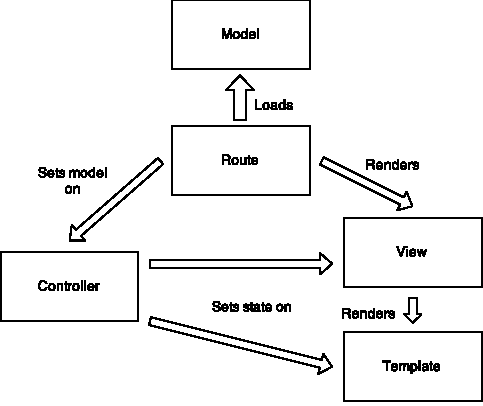
\includegraphics[width=10cm]{1_ember_architecture}
\caption{Ember framework architecture}\label{ember_architecture}
\end{figure}

But for simple applications that do not require these features, Angular or React for example might be an overkill. As new updates come out, supporting the UI might get more and more expensive. For an application with just a few buttons that the user should only interact a few times a year, simple HTML and Javascript should be just enough.

Until now everything discussed was related to building the front part of a modern web application. But a web application usually consist also from the backed part. The HTTP application that listens to client requests. For building one there are a lot of frameworks which allows to scaffold a prototype. MVC based frameworks are powerful and provides lots of functionalities out of the box and the good thing is that the majority of frameworks are mature and stable. Here are a list of frequently used solutions:
\begin{itemize}
    \item Django;
    \item ASP.NET Core;
    \item Ruby on Rails;
\end{itemize}

The mentioned technologies have huge stacks that sometimes are not needed when building a smaller application, or scalable one. Besides for building modern web applications where the client application is developed in a Javascript framework, means that the "V" (view) part from MVC is not needed anymore. Plus there are already on the market lightweight web technologies such as Sinatra, Flask, Node (in combination with express library). This type of application can serve just as good. In case if new module is required by the application, it can be easily added to the micro-framework stack. In ruby this is done by using gemfiles (gems are libraries in Ruby language) were gems can be easily added and installed effortlessly.

\subsubsection{Web Sockets}
WebSocket is a protocol providing full-duplex communication channels over a single TCP connection. The WebSocket protocol was standardized by the IETF as RFC 6455 in 2011, and the WebSocket API in Web IDL is being standardized by the W3C. The WebSocket Protocol is an independent TCP-based protocol. Its only relationship to HTTP is that its handshake is interpreted by HTTP servers as an Upgrade request. The WebSocket protocol makes more interaction between a browser and a website possible, facilitating live content and the creation of real-time games. This is made possible by providing a standardized way for the server to send content to the browser without being solicited by the client, and allowing for messages to be passed back and forth while keeping the connection open. In this way a two-way (bi-directional) ongoing conversation can take place between a browser and the server. The communications are done over TCP port number 80, which is of benefit for those environments which block non-web Internet connections using a firewall. Similar two-way browser-server communications have been achieved in non-standardized ways using stop-gap technologies such as Comet. In DSLR Camera Controller web sockets are used to transfer the live preview from the server.

The WebSocket protocol is currently supported in most major browsers including Google Chrome, Internet Explorer, Firefox, Safari and Opera. WebSocket also requires web applications on the server to support it. WebSocket reduces latency. For example, unlike polling, WebSocket makes a single request. The server does not need to wait for a request from the client. Similarly, the client can send messages to the server at any time. This single request greatly reduces latency over polling, which sends a request at intervals, regardless of whether messages are available. WebSocket makes real-time communication much more efficient. Polling can always be used (and sometimes even streaming) over HTTP to receive notifications over HTTP. However, WebSocket saves bandwidth, CPU power, and latency. WebSocket is an innovation in performance. It is also is an underlying network protocol that enables to build other standard protocols on top of it. It is also a part of an effort to provide advanced capabilities to HTML5 apps in order to compete with other platforms.

\cleardoublepage

\section{Software Design}
\phantomsection

\subsection{UML Modeling}
In the current chapter is represented and described the architecture of DSLR Camera Controller application. It contains a set of relevant diagrams modeled in UML language. The diagrams provide a fundamental documentation an description of the system structure and behavior.

The aspect that should be defined is how the user will interact with the application. Therefore a use case diagram was modeled to show the set of available actions offered at the user's disposal. The client part of the application represents a browser web page. There are six main actions a user can perform. The operations can be seen in \mbox{figure \ref{use_case}}. When the application is opened, the user can view/manage the connected cameras. The seconds main action is to manage a selected camera's settings. The app should detect all available configurations supported by the camera, if it has any. Next, the user can take a photo and get a live preview as well. Additionally, the user is allowed to configure a failure strategy. And finally, the main action is to allow the user to configure a time-lapse.

\begin{figure}[!ht]
\centering
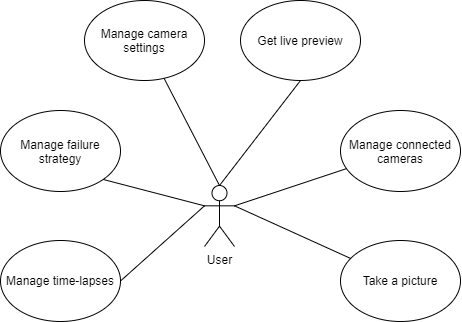
\includegraphics[width=15cm]{2-user-use-case-diagram}
\caption{User use case diagram}\label{use_case}
\end{figure}

To offer a detailed overview of how the entire system works, a set of sequence diagrams are provided. They show key parts of the platform and the way they interact. Moreover it is crucial to depict the depth of chain of events happening in the background. For instance the sequence diagram, shown in \mbox{figure \ref{user_sequence}}, specifies what happens when a user simply asks for camera settings. First of all the client browser does an HTTP request in order to get the application page. Now the user is able to interact with the platform. When the client requests the settings on a detected camera, the application first has to ask the selected camera's available configurations. The camera, if it supports this feature, will return a list of settings. These settings also include read-only configurations, like serial number or camera power, so the application filters the known read-only configurations and returns them to the user.

\begin{figure}[!ht]
\centering
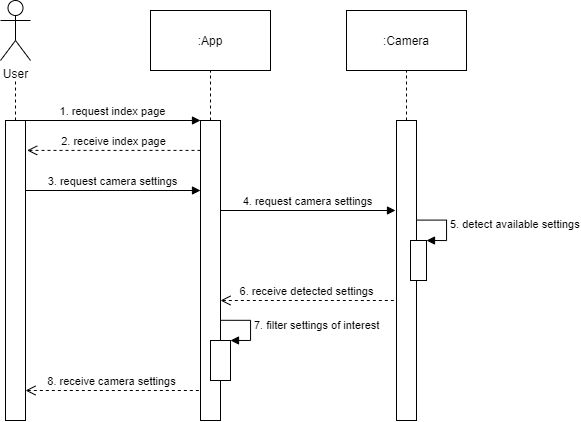
\includegraphics[width=15cm]{2-user-sequence-diagram-get-cam-settings}
\caption{Camera settings sequence diagram}\label{user_sequence}
\end{figure}

For time-lapses we can distinguish two main steps. Each one is described in the sequence diagrams illustrated below. Their behavior looks a bit similar, nevertheless each has unique characteristics worth point out.

The first step of a time-lapse is the process of scheduling one, that is depicted in \mbox{figure \ref{timelapse_request_sequence}}. First, the user requests a new schedule. The most important data that the user has to provide is the \textbf{cron} expression, which is used for scheduling. The request is then processed in the application, so that it is configured to require the currently connected cameras. If a camera is missing during a capture event, the platform will consider it as a failure and will take the appropriate measures (send email notifications, hard reset, etc.). Next, a special worker that runs separately from the main thread receives the request. The worker then registers the new time-lapse into a persistence mechanism and computes its next run based on all available time-lapses. Reading all the active time-lapses from the database is not the most optimal method, but considering that there will usually be only one active time-lapse, it can be considered satisfactory. At the end, the user receives a success message with the newly created schedule.

\begin{figure}[!ht]
\centering
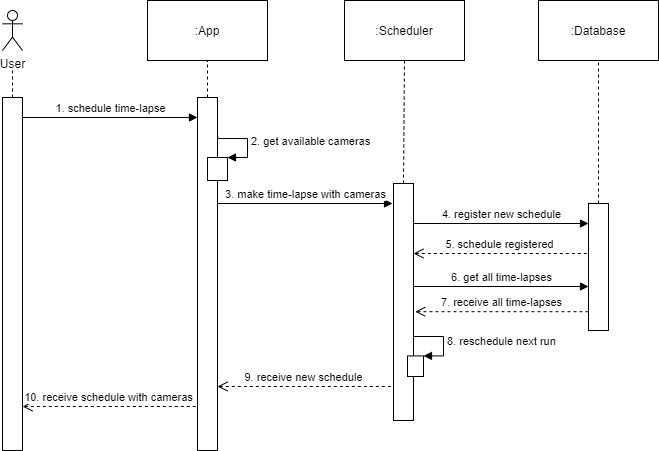
\includegraphics[width=15cm]{2-timelapse-request-sequance-diagram}
\caption{Time-lapse requesting sequence diagram}\label{timelapse_request_sequence}
\end{figure}

The sequence diagram, illustrated in \mbox{figure \ref{timelapse_triger_sequence}}, represents the next step after the user has successfully registered a time-lapse. When the Scheduler triggers a capture event it runs an abstract command composed by the application. This command goes through the list of required cameras and tries to take a picture. After the picture was taken, the scheduler recomputes when it should run the next time. Afterwards, an event that the picture was successfully taken is then published. The application has a special handler for this event which transfers the file if it was configured to do so, then it logs the successful capture and transfer.

\begin{figure}[!ht]
\centering
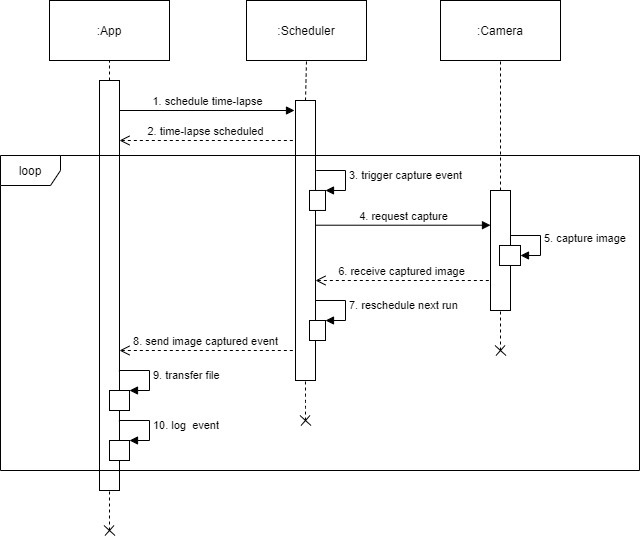
\includegraphics[width=15cm]{2-timelapse-triger-sequance-diagram}
\caption{Schedule capture trigger sequence diagram}\label{timelapse_triger_sequence}
\end{figure}

The time-lapse is the most crucial feature of the application. So, to better understand how it works, in the figure \mbox{\ref{timelapse_iteration_activity}} is described through an Activity Diagram a single iteration of the time-lapse. It starts by rescheduling its next run. When a capture event is published, the application requests the time-lapse's cameras to take a picture. If a camera is missing, or one of the cameras returned an error, or some error happened, the application registers it as an error. The details of the failure are registered in a special logging system that the user can later query from the web. Afterwards the failure process starts. Otherwise, if there were no errors while taking photos, the photo is logged and then the file transfer routine starts, independent of photo capturing routines. Again, if an error occurs in this step, it is also logged in the system.

\begin{figure}[!ht]
\centering
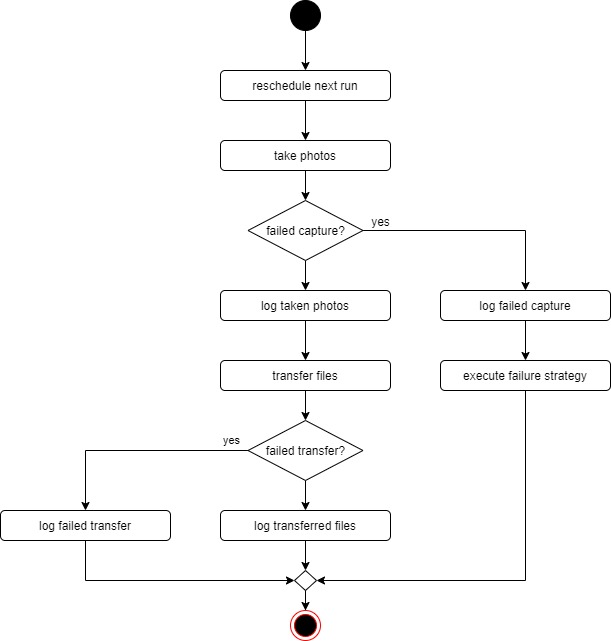
\includegraphics[width=14cm]{2-time-lapse-iteration}
\caption{Time-lapse iteration activity diagram}\label{timelapse_iteration_activity}
\end{figure}

The processing of the capture failures is a key feature of this application as well. Coming up with a few practical solutions that would work across multiple camera models was not an easy task. Nevertheless, in the figure \mbox{\ref{timelapse_failure_activity}} is described the activity diagram of how the failures are being handled. This is an extension of the diagram from the figure \mbox{\ref{timelapse_iteration_activity}}. First, if the user has enabled the email notification feature, on failure, the application will fetch all the emails registered for notifications and send them the error message. Then, if hard resetting is enabled, the application will first try to programmatically reconnect to the cameras. In some cases this is good enough, as some camera models simply require a wake-up call. Then, if an Ykush device is detected to be connected to the system, then it activates it as well, which basically re-plugs the cameras. Re-plugging almost always solves any problems it might have encountered. And finally, if system rebooting is enabled, the program will reboot the system after a consecutive number of failures. This allows the user to reset the USB connections at the expense of processing time. But considering that it is cheaper than an external device for reconnecting the USB connections, this may be viable enough option as well.

\begin{figure}[!ht]
\centering
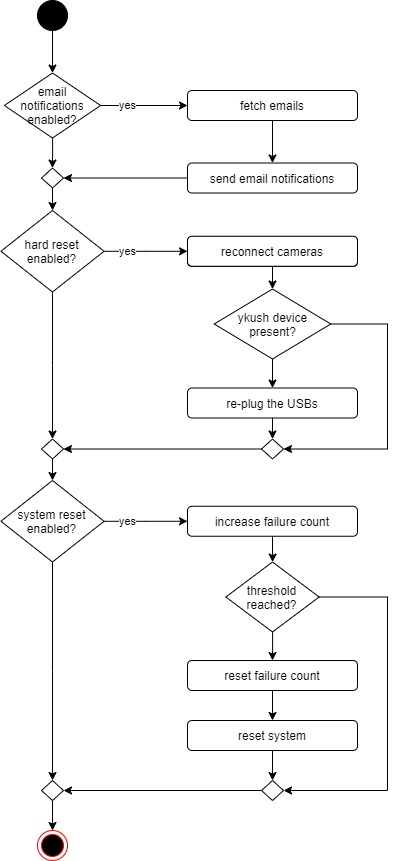
\includegraphics[width=7cm]{2-timelapse-failure-activity}
\caption{Time-lapse failure activity diagram}\label{timelapse_failure_activity}
\end{figure}

In the following part of this chapter is described the most important classes of the DSLR Camera Controller application through a few class diagrams. Most of them are related to the camera and time-lapse management. Information about the system components interaction is not enough for understanding the tool. The class diagrams deliver information under a higher level of granularity, hence the system becomes more easy to comprehend.

First in the figure \mbox{\ref{camera_manager_class_diagram}} is described how the application is using the cameras. The concept of camera is completely abstracted from the core. The whole application simply communicates with an abstract camera that is known to have a few functionalities like capturing an image, setting a configuration, etc.. Binding the application to the fact that the cameras are connected through some ports or that it is using a special library to communicate with the camera would transform the maintenance of the application into a nightmare. That's why the implementation of the abstract camera and camera manager sits in the infrastructure level of the application. To allow testing of some functionalities without any cameras connected, some fake cameras were introduced with a few predefined configurations like output image, available setting, etc.. CameraManager works with cameras, but the implementations are aware what kind of cameras they are working with, so it is not quite the Bridge design pattern implemented here.

\begin{figure}[!ht]
\centering
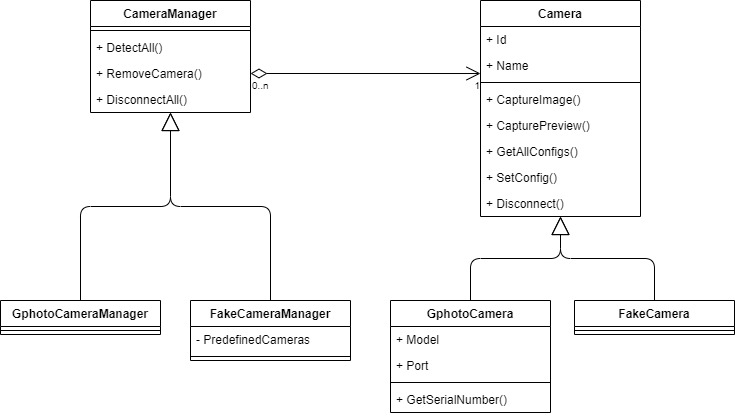
\includegraphics[width=18cm]{2-camera-manager-class-diagram}
\caption{Camera management class diagram}\label{camera_manager_class_diagram}
\end{figure}

Next follows a class diagram on how a time-lapse is persisted on the platform. In the figure \mbox{\ref{timelapse_data_class_diagram}} is represented what data is required for a time-lapse. It is composed of a nullable schedule and has reference to the required cameras. If the schedule is null, then it means that the time-lapse has been put on hold. The separation of the time-lapse from the schedule offers the possibility to reuse the scheduling logic for other features. One of the requested feature was to email a monthly report on the progress of the application.

\begin{figure}[!ht]
\centering
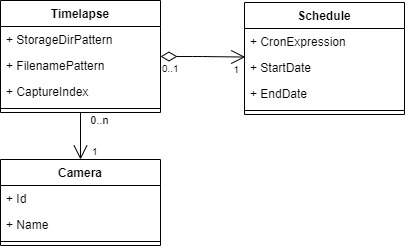
\includegraphics[width=13cm]{2-timelapse-data-class-diagram}
\caption{Time-lapse data class diagram}\label{timelapse_data_class_diagram}
\end{figure}


% The platform modules and their behavior were described until now. Another important part of the application is the set of libraries it uses and their purpose, depicted in \mbox{figure \ref{component_diagram}}. Because the project is divided in two parts there are two set of dependencies and libraries. The data mining part is a console applications, hence the set of required libraries is small. The essential library is rest\_client, used for requesting web pages and getting their content. Nokogiri is used for parsing HTML and extracting the necessary elements. Savon is a library for SOAP communications, needed for NLP processing. Mongoid is used for database communication, as it was discussed above. The client part of application requires more libraries because it consists from more logical components. Some gems (a ruby term for library) are shared between the logical components, for example Mongoid. Sinatra framework is used to build the web applications. The main goal is to handle client's HTTP requests. Faye library is used to host the websocket server. It is handy because it provides a higher level of functionality than a simple websocket. Haml gem aims to process the haml files for creating web page content. Haml is a dialect of HTML, simply put another markup language. Sidekiq is a library used for running asynchronous jobs. Redis is a dependency required by Sidekiq and it is used as a message queue system. D3 is a JavaScript library used for drawing plots and charts. This sums it up. Of cores there are also other dependency libraries.

% \begin{figure}[!h]
% \centering
% 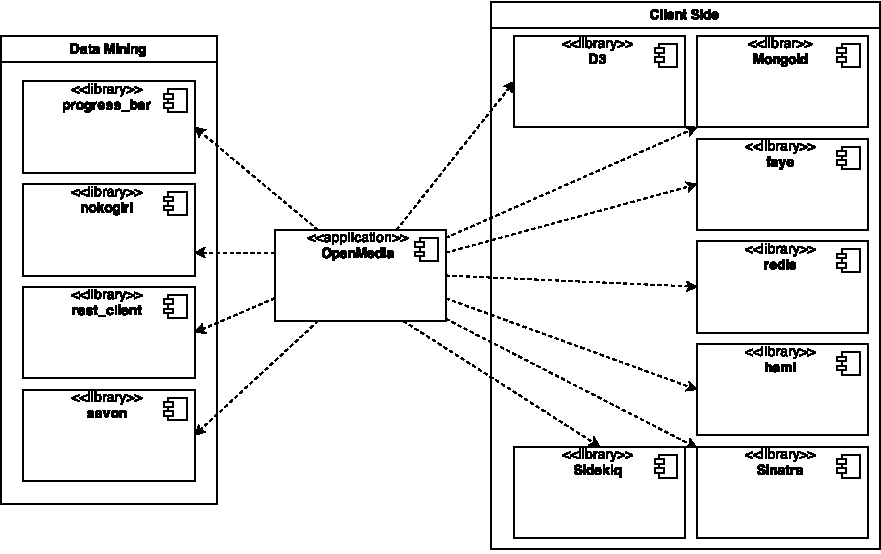
\includegraphics[width=16cm]{2_component_diagram}
% \caption{Component diagram of OpenMedia}\label{component_diagram}
% \end{figure}

% The deployment diagram gives a good understanding of the whole system. OpenMedia platform has a complex structure and consist of more than a few modules, see \mbox{figure \ref{deployment}}. In order to launch the application, not every module needs to be up and running. Data mining application is a console ruby applications which only requires to run once in a while in order to keep the database content up to date. Moreover the NLP server is an external web service maintained by \emph{Institutul de Cercetare pentru Inteligență artificială Mihai Drăgănescu, Academia Română}. The diagram shows in details the complexity of OpenMedia platform. It also depicts the ways of communication between logical units of the application, concluding that some modules not only communicate with multiple entities, they also use different communication protocols. For instance Sinatra and Sidekiq servers communicates with three modules each, where the communication protocols are Mongoid API, Redis API, and the HTTP protocol. Another aspect is the operating systems used by every component. Linux is the main operating system for most of the modules. Regarding the client application, the operating system doesn't matter as long as it has installed a modern web browser. For Racai web service the operating system is unknown. This proves how powerful are the web services. A developer is not concerned about the internal infrastructure of the web service. As long as it complains a standard protocol a successful communication is achieved.

% \begin{figure}[!ht]
% \centering
% 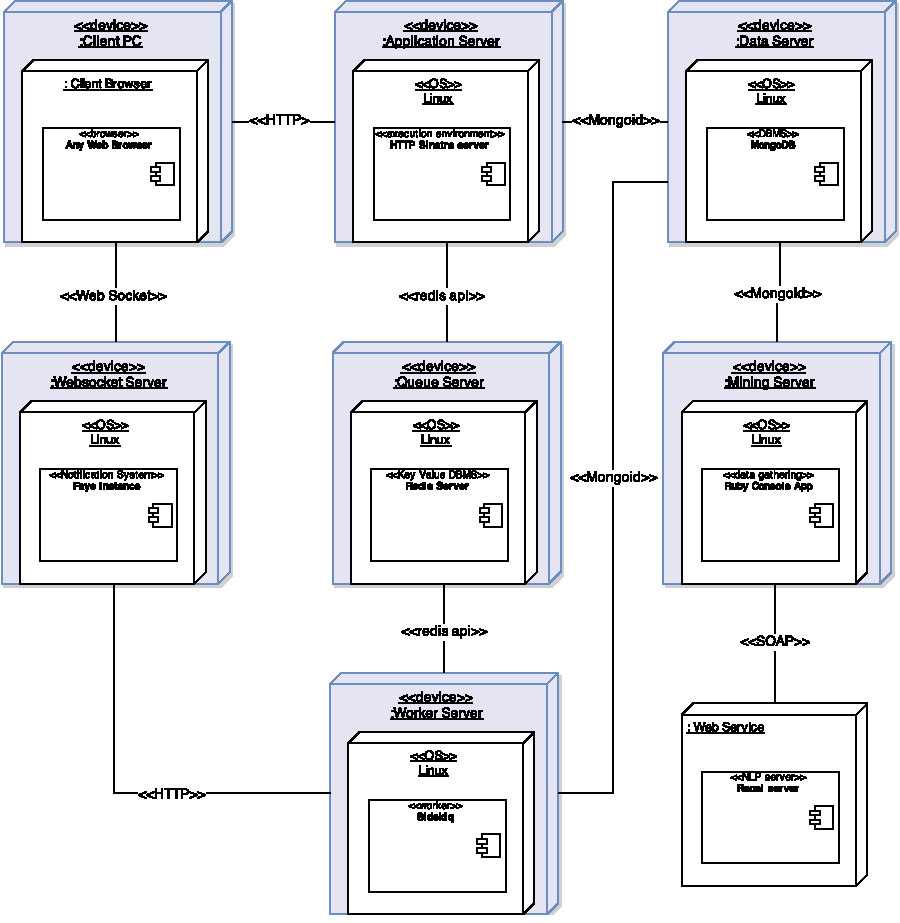
\includegraphics[width=18cm]{2_deployment}
% \caption{OpenMedia deployment diagram}\label{deployment}
% \end{figure}

% Therefore the UML diagrams concentrate on the application prototype. They cover the most useful standard diagrams: use case diagrams, sequence diagrams, class diagrams, state diagrams, activity diagrams, components diagrams and deployment diagrams. All diagrams express the relationships, structural and behavioral aspects of the system. Modeling the application is for more reasons. The first and the obvious one, is to communicate the application architecture and its behavior. But the important aspect is, while modeling the platform the problem is understood better.

% The implementation chapter focuses on the provided UML design, implements the classes and follows the use cases and sequence diagrams to define the flow of the application. The application components and dependencies will probably extend to a bigger degree. This concludes the UML description of the project, that aimed at presenting the most relevant aspect of the system and covering the general architecture of the application. The UML methodology offered a good documentation basis and a clear view on requirements of the software.
\cleardoublepage

\section{Implementation Part}

\phantomsection
In the previous chapters were discussed the concepts covered by DSLR camera controlling project. The research of the ideas is crucial given that the applications aims a niche that is relatively new in the market. To be sure that the platform development start from the right foot, a thorough architecture design, modeled in UML language, was provided in the previous chapter. What follows now is the description of the implementation part. An exhaustive description of every step will be given, including code snippets, the technologies used and the reason of their choice.

\subsection{Used Tools}
In order to achieve a better performance in this application development, there were choose specific tools that are offering the possibility to implement and extend the application's functionality.

\vspace{0.3cm}
\textbf{PyCharm}

PyCharm brings you a smart coding assistance for Python languages, Javascript, HTML and CSS. Enjoy code completion, powerful navigation features, on-the-fly error detection, and refactoring assistance for all of these languages. PyCharm provides advanced coding assistance for Django, Angular, Javascript and more. All in one IDE. The IDE analyzes your project to provide the best code completion results for all supported languages. Hundreds of built-in inspections report any possible issues right as you type and suggest quick-fix options. PyCharm helps you get around your code more efficiently and save time when working with large projects. Jump to a method, function or variable definition in just one click, or search for the usages.It also supports advanced features like remote SHH project development and a lot more.

PyCharm provides powerful built-in tools for debugging, testing and tracing your server-side and client-side applications. With minimum configuration required and thoughtful integration into the IDE, these tasks are much easier with PyCharm. Place the breakpoints, step through the code, and evaluate expressions – all without leaving the IDE.

PyCharm integrates with popular command line tools for web development, providing you with a productive, streamlined development experience without using the command line. PyCharm (community edition) is built on top of the open-source IntelliJ Platform, which JetBrains have been developing and perfecting for over 15 years. Enjoy the fine-tuned, yet highly customizable experience it provides to fit your development workflow. PyCharm provides a unified UI for working with many popular Version Control Systems, ensuring a consistent user experience across git, GitHub, SVN, Mercurial, and Perforce. PyCharm is extremely customizable. Adjust it to perfectly suit your coding style, from shortcuts, fonts and visual themes to tool windows and editor layout. \cite{pycharm}\vspace{0.3cm}

\textbf{gPhoto}

gPhoto is a set of software applications and libraries for use in digital photography. gPhoto supports not just retrieving of images from camera devices, but also upload and remote controlled configuration and capture, depending on whether the camera supports those features. Released under the GNU Lesser General Public License, gPhoto is free software.

gPhoto supports more than 2500 cameras as of June 2019. It is cross-platform, running under Linux, FreeBSD, NetBSD and other Unix-like operating systems.

gPhoto has support for the Picture Transfer Protocol (PTP) and will also connect to devices that use the Media Transfer Protocol (MTP). Many cameras are not supported by gPhoto, but have support for the USB mass storage device class, which is well-supported under Linux.

gPhoto supports camera tethering control, preview, viewfinder in PTP or camera specific protocols on numerous cameras. \cite{gPhoto}

\vspace{0.3cm}
\textbf{SSH}

For a quick, cheap and secure connection with the system that has the cameras connected, SSH brings all the required tools to ease the use and management of the \ThesisTitle.

Secure Shell (SSH) is a cryptographic network protocol for operating network services securely over an unsecured network. Typical applications include remote command-line, login, and remote command execution, but any network service can be secured with SSH.

SSH provides a secure channel over an unsecured network by using a client–server architecture, connecting an SSH client application with an SSH server. The protocol specification distinguishes between two major versions, referred to as SSH-1 and SSH-2. The standard TCP port for SSH is 22. SSH is generally used to access Unix-like operating systems, but it can also be used on Microsoft Windows. Windows 10 uses OpenSSH as its default SSH client and SSH server.

SSH was designed as a replacement for Telnet and for unsecured remote shell protocols such as the Berkeley rsh and the related rlogin and rexec protocols. Those protocols send information, notably passwords, in plaintext, rendering them susceptible to interception and disclosure using packet analysis. The encryption used by SSH is intended to provide confidentiality and integrity of data over an unsecured network, such as the Internet, although files leaked by Edward Snowden indicate that the National Security Agency can sometimes decrypt SSH, allowing them to read, modify and selectively suppress the contents of SSH sessions. \cite{ssh}

\vspace{0.3cm}
\textbf{YKUSH Yepkit}

YKUSH boards allow the user to selectively switch ON and OFF the power of each of the USB devices connected to the Hub downstream ports. The control is done using an application in the host system (e.g., PC to which the YKUSH board is connected. Switching ON/OFF a YKUSH downstream port with a device connected to it has the same effect as to physically Connecting/Disconnecting a Device to a port of a typical USB hub.

The switching control is performed by sending commands to the on-board micro-controller (YKUSH board control unit), which is seen by host as a HID USB device not requiring the installation of specific drivers. The communication between the host and the board control unit is based on a simple message protocol. The communication protocol is documented and detailed in the Product Manual available for download bellow, in the Documents and Resources section. \cite{yepkit}

\vspace{0.3cm}
\subsection{Camera abstractions}

Dependency Inversion principle is as simple as it is important: High-level modules, which provide complex logic, should be easily reusable and unaffected by changes in low-level modules, which provide utility features. From Bob Martin's definition, it mentions that abstractions should not depend on details. Details should depend on abstractions \cite{solid-d} \cite{uncle-bob-book}. An important detail of this definition is, that \textbf{high-level} and \textbf{low-level} modules depend on the abstraction.

\vspace{0.3cm}
Following this principle, it was important to distinguish which parts of this application should be treated as details. It may not be obvious at first, but after a through investigation the camera and all its management can be treated as an abstract concept. Following the same principle, we can distinguish a few abstractions worth noting:
\begin{itemize}
    \item Camera \& Camera management (gPhoto);
    \item Camera reset logic (Ykush);
    \item Scheduling (Django scheduling);
    \item File transfer (rsync);
\end{itemize}

\vspace{0.3cm}
From an architectural point of view, a DSLR camera is a detail. The fact that gPhoto tool is used to communicate with cameras is also a detail. To avoid tightly coupling the \textbf{Business} to such details, making it hard to change, it's important to abstract the core logic from it. In the \textbf{\mbox{listing \ref{camera_interface}}} it is represented the general interface of a camera. The 2 most important functionalities are: get/set config and capture image. It also has preview capturing for getting a quick lightweight preview of the camera, useful for live previewing.

\vspace{0.3cm}
\lstinputlisting[language=Python, caption={Camera Interface}, label=camera_interface]{../src/camera.py}

\vspace{0.3cm}
To facilitate the communication with all the connected cameras, a Camera Manager is introduced. It is designed to abstract the orchestration of cameras in a way that the user would not need to know anything about the synchronization problems gPhoto has. In the \textbf{\mbox{listing \ref{camera_manager_interface}}} it is represented a rough summary of what this manager is expected to be able to do.

\vspace{0.3cm}
\lstinputlisting[language=Python, caption={Camera Manager Interface}, label=camera_manager_interface]{../src/camera_manager.py}

\vspace{0.3cm}
Inspecting the requirements, the client was in a need for a small but powerful functionality. He would need to quickly detect all connected cameras. Therefore, a \textit{detect all cameras} functionality is requested from the manager. After the cameras are detected, the \textit{cameras} property should be filled with \textit{Camera} instances. This would allow the user to iterate through all the detected cameras an run the required functionality.

\vspace{0.3cm}
To have a serializable method of communicating between the user and the system, a unique Id is required. The concrete cameras are expected to expose a unique identifier which would allow the user to query a specific camera from the manager. The user would then be able to remove a camera from the manager if required.

\vspace{0.3cm}
\subsection{Camera implementations}
Being able to test the application without any connected cameras brings a large range of benefits, some of them would be:

\begin{itemize}
    \item Independent development of the client side;
    \item Stress testing;
    \item Less budget consumption for camera renting;
\end{itemize}

\vspace{0.3cm}
This brings us to the conclusion that a fake camera would perfectly fit for the development of this application. A more technical name for such a concept would be a \textit{test stub}. In advanced polymorphism computer science, test stubs are programs that simulate the behaviours of software components that a module undergoing tests depends on. Test stubs are mainly used in incremental testing's top-down approach \cite{test-stub}. Additionally, these stubs will also help in testing if the right abstractions were made, helping in developing a more robust and reliable architecture which would drastically help in further development.

\vspace{0.3cm}
In the \textbf{\mbox{listing \ref{stub-img-capture}}} is represented a piece of code of how these stubs work. Mainly, the constructor receives all the required information, otherwise it auto-generates predefined data. For example, when a preview or image is requested, it simply draws two triangles using the \textit{pillow} library for drawings.

\vspace{0.3cm}
\lstinputlisting[language=Python, caption={Stub image capture}, label=stub-img-capture]{../src/stub_capture_img.py}

\vspace{0.3cm}
Next, in the \textbf{\mbox{listing \ref{gp-detect-all}}} it is represented how \textit{gPhoto} tool is used to detect all detected cameras.

\vspace{0.3cm}
\lstinputlisting[language=Python, caption={gPhoto detect all cameras}, label=gp-detect-all]{../src/gp_detect_all.py}

\vspace{0.3cm}
\textit{gPhoto} is a very fragile library. It may sometimes work on OSX but fail to run some simple commands on the Linux environment. To avoid any unforeseen bugs and to simply ease the development process, a synchronization system was introduced. This system would only allow a single caller to communicate with the cameras, otherwise the library usually fails (this is in regard to \textit{\_gp\_lock}).

\vspace{0.3cm}
Detecting all cameras is quite simple using \textit{gPhoto}. The first step is to ensure that all cameras are disconnected. Next, it gets all the camera names and ports. Afterwards, information about the available ports are loaded. Finally, depending on the port and the loaded information, the \textit{GpCamera}s are created. \textit{GpCamera} is a concrete implementation of \textit{Camera}. Now, the user can simply iterate through the cameras and execute the required functionality.

\vspace{0.3cm}
Now, the most important functionality is represented in the \textbf{\mbox{listing \ref{gp-capture-img}}}. The entire application relies on this specific functionality, therefore it became slightly sophisticated.

\lstinputlisting[language=Python, caption={gPhoto capture image}, label=gp-capture-img]{../src/gp_capture_img.py}

\vspace{0.3cm}
Before starting any communication with the camera, a lock is put in place to prevent any other threads from interfering. Then, a new connection is open. Next, the \textit{gPhoto} library captures an image with the preset settings and saves it on the local storage. Then the next step is to move it on the current system, which is also done through \textit{gPhoto}. When the file is moved, it is given a new name which follows the complex file naming requirements described earlier. And finally, the full path of the new image on the local system is returned.

\vspace{0.3cm}
While image capturing might seem a big overwhelming at first, preview capturing on the other hand is much more simple. In the \textbf{\mbox{listing \ref{gp-capture-preview}}} it is represented how this process is taken care of.

\lstinputlisting[language=Python, caption={gPhoto capture preview}, label=gp-capture-preview]{../src/gp_capture_preview.py}

\vspace{0.3cm}
Since the file is lightweight and short living, it is read in memory and returned, therefore no additional tasks are required. This makes live previewing a lot faster than trying to store it on the local storage.

\vspace{0.3cm}
\subsection{Scheduling}

Creating a schedule was never an easy task. Initially the client required a very specific use case: "A schedule that triggers camera capture every minute or so from Monday to Friday, from 8 AM until 8 PM". Using timers for this use case would easily solve the problem. But then, the client may want a whole different type of schedule. For example, he may require a schedule that would trigger the capture event every second day, or a schedule with lunch breaks, etc.. This would create a whole lot of additional unnecessary complications. For every new type of schedule, the scheduling part would need to be modified.

To not reinvent the wheel, the best tool for this job became \textit{cron}. This software utility is a time-based job scheduler in Unix-like computer operating systems. Users that set up and maintain software environments use cron to schedule jobs (commands or shell scripts) to run periodically at fixed times, dates, or intervals. It typically automates system maintenance or administration—though its general-purpose nature makes it useful for things like downloading files from the Internet and downloading email at regular intervals. The origin of the name cron is from the Greek word for time chronos. Cron is most suitable for scheduling repetitive tasks. Scheduling one-time tasks can be accomplished using the associated \textit{at} utility \cite{cron}.

Using the \textit{apscheduler} python library allows the use of this very tool to create schedules. The \textbf{\mbox{listing \ref{cron-schedule}}} contains the definition of a cron schedule used in this application.

\lstinputlisting[language=Python, caption={Cron schedule}, label=cron-schedule]{../src/cron_schedule.py}

\vspace{0.3cm}
Again, to allow the use of different tools other than \textit{apscheduler}, the business logic defines an abstraction over the scheduling process which is represented in the \textbf{\mbox{listing \ref{cron-scheduler}}}.

\lstinputlisting[language=Python, caption={Cron scheduler}, label=cron-scheduler]{../src/cron-scheduler.py}

\vspace{0.3cm}
The start method would be used for starting all the existing schedules. For example \textit{apscheduler} works by reading and writing to a predefined persistence mechanism. In \ThesisTitle it is configured to use a lightweight SQLite database. This allows persisting the jobs even when the application is forcefully stopped or a power outage happens, which is a critical sale point for this application. As described earlier, the existing applications had trouble automating this part. In the \textbf{\mbox{listing \ref{cron-scheduler}}} it is described the implementation of the \textit{apscheduler}.

\lstinputlisting[language=Python, caption={Aps Scheduler implementation}, label=aps-scheduler]{../src/asp_cheduler.py}

\vspace{0.3cm}
At the start, it configures to use the \textit{DjangoJobStore} which simply tells the scheduler to use the same persistence mechanism as defined in Django. Basically, instead of directly referencing the library from the core, the core application defines an interface which is latter implemented by a third party library. In other words \textit{ApsScheduler} is a wrapper around library's own scheduler.

Using such a tool brings its own risks and complications though. The user would need to learn a bit how to define cron expressions. For this reason, this part must be thoroughly documented so that it's much easier to get started. 

\vspace{0.3cm}
\subsection{Web API}

For the web part, the application uses the Django framework. It is an open-source python web framework used for rapid development, pragmatic, maintainable, clean design, and secures websites. Django is a Python-based free and open-source web framework that follows the model-template-view (MTV) architectural pattern. It is maintained by the Django Software Foundation (DSF), an American independent organization as a non-profit organization \cite{django}.

Each \textit{view} represents a specific use case of the application. Each such use case is separated in its own class making development independent of other views. For resolving the required dependencies, the Dependency Injection principle is used. In software engineering, dependency injection is a technique in which an object receives other objects that it depends on. These other objects are called dependencies. In the typical "using" relationship the receiving object is called a client and the passed (that is, "injected") object is called a service. The code that passes the service to the client can be many kinds of things and is called the injector. Instead of the client specifying which service it will use, the injector tells the client what service to use. The "injection" refers to the passing of a dependency (a service) into the object (a client) that would use it \cite{di}. For dependency injection, the application uses \textit{pinject} tool which is a is a dependency injection library for python \cite{pinject}.

The \textbf{\mbox{listing \ref{capture-img-view}}} represents how Django uses the application's core functionality to expose an API. The routing for this view is latter configured in a Django setting file.

\lstinputlisting[language=Python, caption={Capture image View}, label=capture-img-view]{../src/camera_capture_img_and_download.py}

\vspace{0.3cm}
First, this view resolves the \textit{CameraCtrlService} from the object graph (\textit{pinject}). Then it tries to call the capture image functionality from the service, returning a FileResponse which is basically a downloadable file for the end user. In case of a failure, like camera is not found or an internal camera error, a respective error is returned to the user.


\vspace{0.3cm}
For live previewing a slightly different approach was taken. Instead of simply returning the current preview, a \textit{StreamingResponse} is returned, which allows endlessly streaming camera previews. The \textbf{\mbox{listing \ref{live-preview-view}}} represents the view for the live preview source.

\lstinputlisting[language=Python, caption={Live preview View}, label=live-preview-view]{../src/camera_preview_source.py}

Sending a big file in Django would best be to stream it in chunks. Similarly, instead of streaming chunks of a file, it streams camera previews in an endless loop, which is automatically canceled on user's request. As a result, the HTML for this functionality becomes very simple and transparent, which can be seen in the \textbf{\mbox{listing \ref{live-preview-template}}}.

\lstinputlisting[language=HTML, caption={Live preview HTML}, label=live-preview-template]{../src/live_preview.html}
\cleardoublepage

\section{Testing and documenting the system}

\phantomsection

Software Testing is necessary because we all make mistakes. Some of those mistakes are unimportant, but some of them are expensive or dangerous.   We need to check everything and anything we produce because things can always go wrong – humans make mistakes all the time.  There is nothing better than a strongly tested software.  Imagine that you spent a lot of time developing something that is not gone used by real users because it’s buggy.  Since we assume that our work may have mistakes, hence we all need to check our own work.\vspace{0.3cm}

However some mistakes come from bad assumptions, so we might make the same mistakes when we check our own work as we made when we did it. So we may not notice the flaws in what we have done. One of the most important things to do if you want to have a successful release and to promote an application and make it popular is to permanently monitor the crash rate of the application and keep it as small as it’s possible.  Because nobody likes when the application is crashing or when something is not working as it’s supposed.But how to keep the crash rate of an application small? Ideally, we should get someone else to check our work because another person is more likely to spot the flaws. \cite{unit-test} \vspace{0.3cm}

But usually, in startups, there is not enough money to pay for human resource and to have quality engineers that will test the application manually and will assure it’s quality. That’s why a good solution would be to have a crash-free application by writing unit tests, instrumentation tests, snapshot tests which were done for the system and will be described below.\vspace{0.3cm}

\textbf{Application's views}

In this section it will be explained how the application works and what the user is able to do with this application. It will be explained all the use cases, starting from camera listing to time-lapse management.

\vspace{0.3cm}
\begin{figure}[!ht]
   \centering
   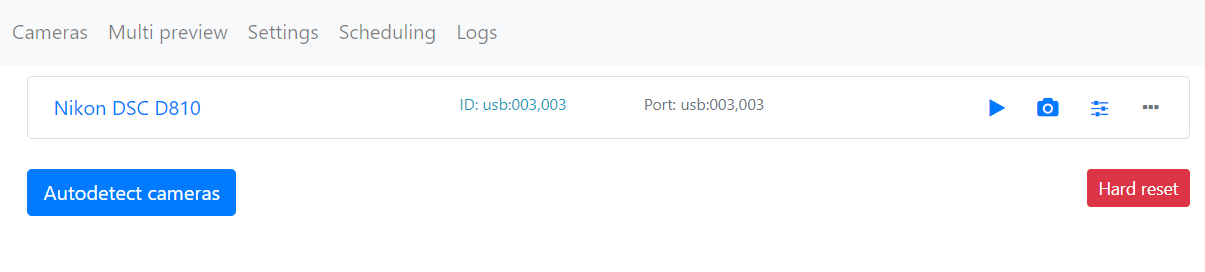
\includegraphics[width=17cm]{test-and-doc/main-view}
   \caption{Application's main page}\label{app-main-view}
\end{figure}

In the \mbox{Figure \ref{app-main-view}} it is represented the first screen the user sees. On the application start-up, the system automatically auto-detects all the cameras, so the user should see a list of the detected cameras. Each listing comes with its own set of buttons, like live preview, image capture, camera settings and camera reconnect. It also displays its Name, ID and the connected port. From this page, the user can re-detect the cameras or hard reset the ports. The hard resetting logic works by triggering the Ykush board if available. This board would then reset the USB ports which effectively re-plugs the USB ports.

\vspace{0.3cm}
\begin{figure}[!ht]
   \centering
   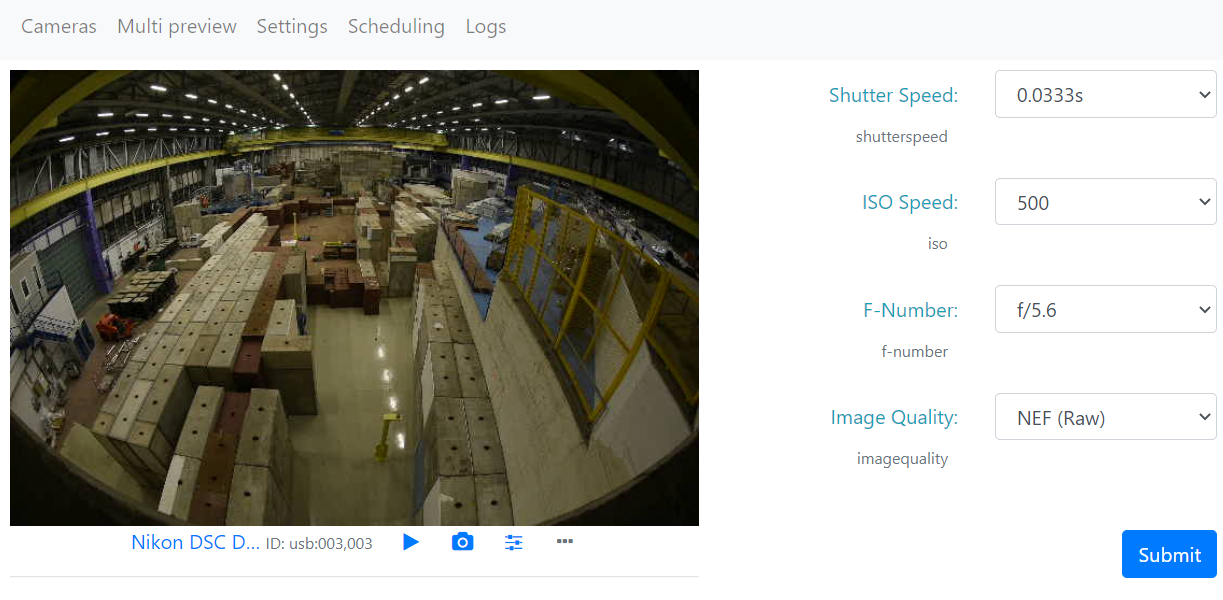
\includegraphics[width=17cm]{test-and-doc/live-preview}
   \caption{Camera live preview}\label{live-preview}
\end{figure}


\mbox{Figure \ref{live-preview}} shows the page containing the live preview of a camera. On the right side is a list with all the favorite settings. These are settings which the user may choose to display on the live preview page.

\vspace{0.3cm}
\begin{figure}[!ht]
   \centering
   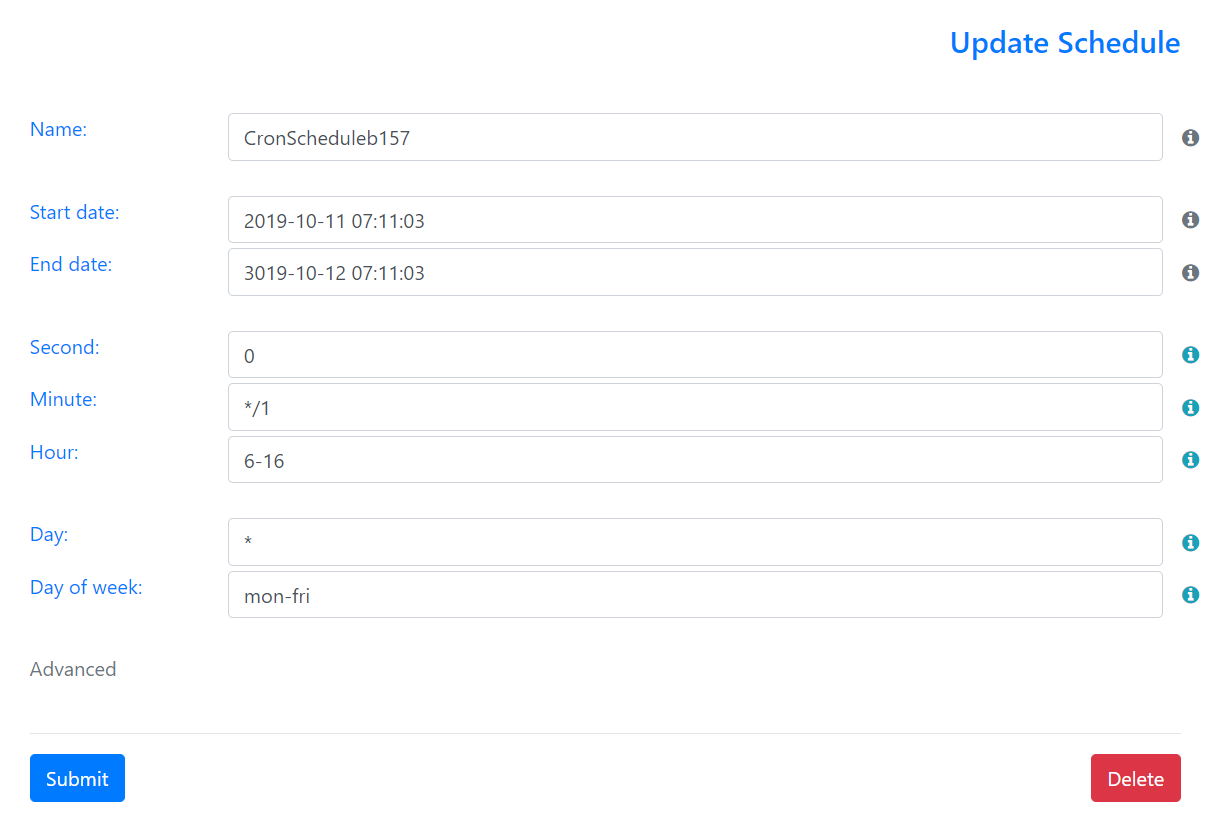
\includegraphics[width=16cm]{test-and-doc/cron-scheduling}
   \caption{Cron scheduling}\label{cron-scheduling}
\end{figure}

In the \mbox{Figure \ref{cron-scheduling}} it is represented the page where the user can configure a schedule. It's not seen in this figure, but below the Submit and Delete buttons the user can find documentation on how to correctly create or modify a schedule.

\vspace{0.3cm}
\begin{figure}[!ht]
   \centering
   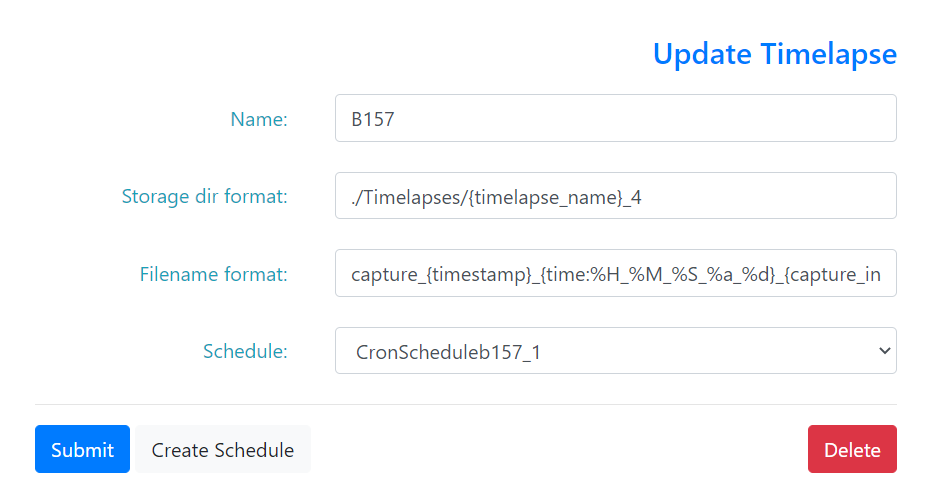
\includegraphics[width=16cm]{test-and-doc/timelapse-scheduling}
   \caption{Time-lapse scheduling}\label{timelapse-scheduling}
\end{figure}

In the \mbox{Figure \ref{timelapse-scheduling}} it is represented the page for Time-lapse configuration. The user can choose the storage directory format and the filename format. Not included in this figure, but if the user scrolls down, he would find some documentation on how to use these features. In this figure for example, the user chose to store the time-lapse photos with a filename that will contain the timestamp, the current time (in the specified format) and capture index. This format produces images in the following form:

\begin{center}
   \verb|B157_4/capture_1591376340024355_16_59_00_Fri_05_94639.nef|
\end{center}

\vspace{0.3cm}
\begin{figure}[!ht]
   \centering
   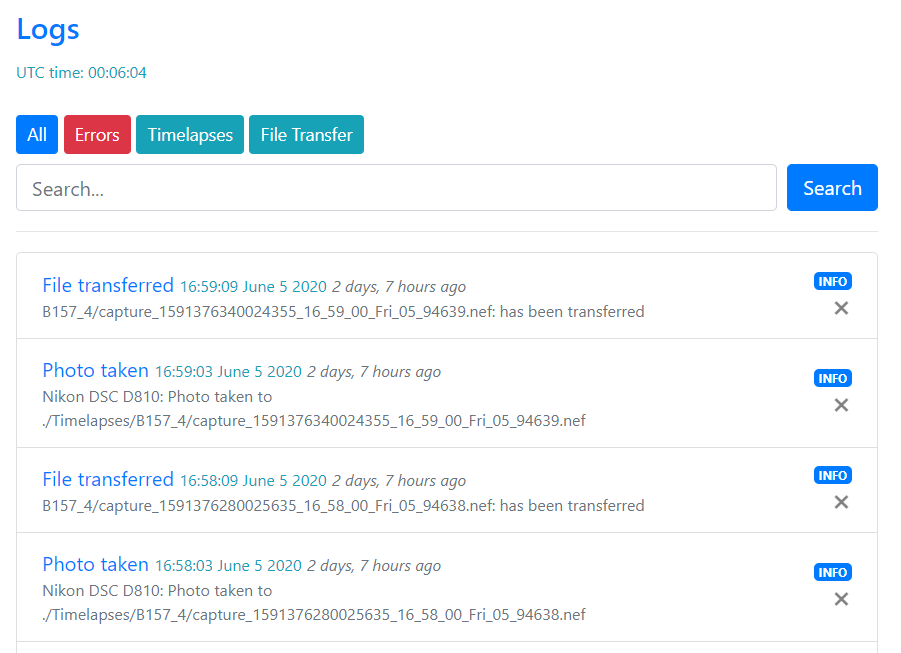
\includegraphics[width=16cm]{test-and-doc/logs}
   \caption{Logs stream}\label{logs}
\end{figure}

In the \mbox{Figure \ref{logs}} it is represented the page containing the stream of logs. Here the user can search and filter specific logs. For example he may choose to display all the errors (which is usually the case). This allows the user to see the progress of how the application is doing.

\vspace{0.3cm}
\begin{figure}[!ht]
   \centering
   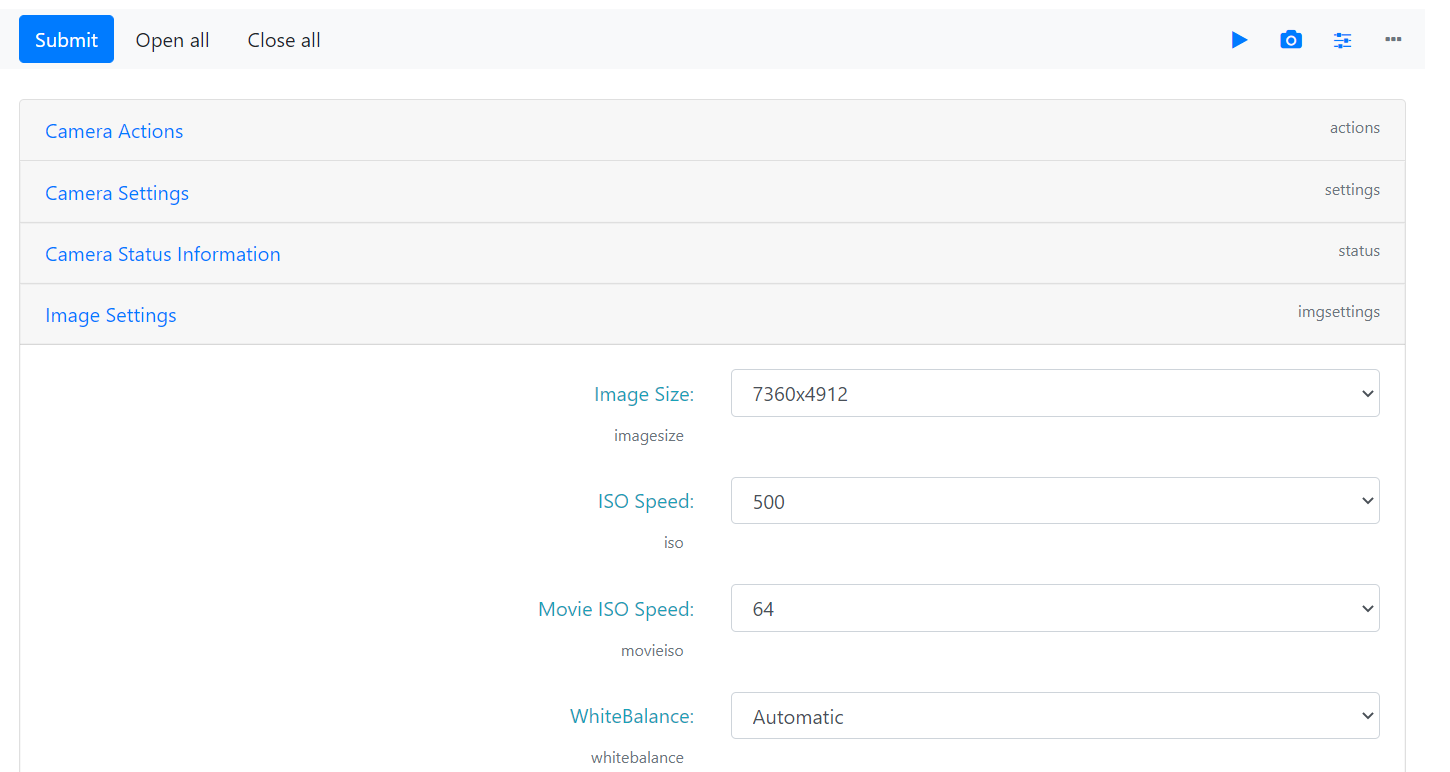
\includegraphics[width=16cm]{test-and-doc/camera-settings}
   \caption{Camera settings}\label{camera-settings}
\end{figure}

And finally, in the \mbox{Figure \ref{camera-settings}} the user can configure any of the available settings. Since \textit{gPhoto} works on a large variety of camera models, some of the displayed fields may be only read-only, that's why when a setting fails to change, an alert next to that setting appears.

\cleardoublepage

\section{Economic Analysis}\label{sec:economy}
\phantomsection

\subsection{Project description}
This section covers the analysis of the developed product from an economic point of view. This product is a web application which whose aim is to facilitate the process of automatically taking long term time-lapses with DSLR Cameras. This section describes aspects like the usefulness of the product, market research, project and time schedule as well as the profitability of the implemented solution.

\subsection{Project time schedule}
The success of the project depends on the right establishing of time constrains of involved activities
as well as resources involved in those activities. For the accomplishment of a project it is necessary to establish a schedule. For the development of the DSLR Camera Controller application, Agile project management is applied to offer flexible and iterative method of designing the application. It goes in 6 stages: requirements, design, develop, test, deploy and feedback. These steps are represented in the figure \mbox{\ref{agile}}. It is a set of repetitive actions which were proven to have a substantial effect on the development of a product.

\begin{figure}[!ht]
\centering
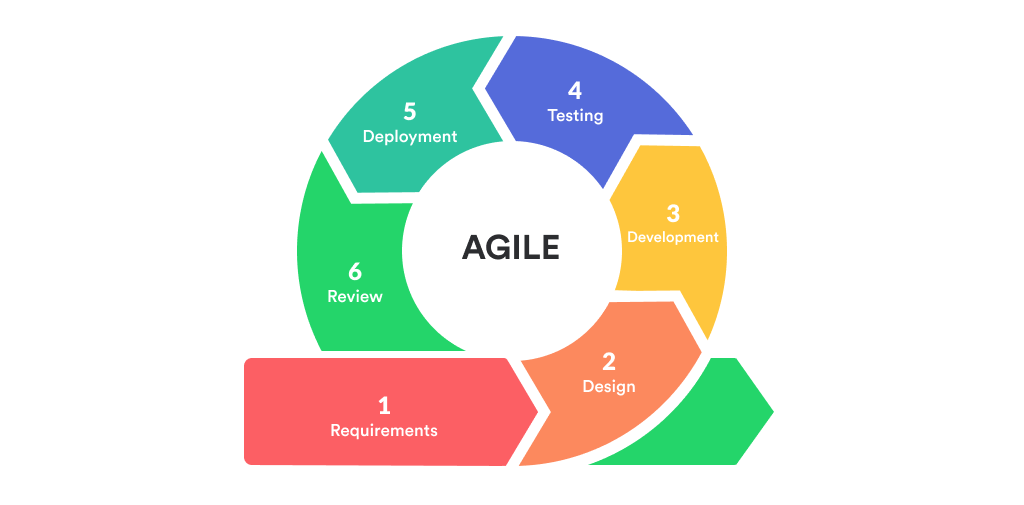
\includegraphics[width=15cm]{4-agile-chart}
\caption{Agile development}\label{agile}
\end{figure}

\subsubsection{Objective determination}
The main objective of the following project is to provide a complete and functioning application for photographers. Otherwise without a finished product there can be no profit. More to that, it is important to market the application and get exposed to a large audience in need. This can be done by targeting first the company that has originally proposed this project.

As it was originally a project requested by the photographic department of CERN (the European Organization for Nuclear Research), this company will prove to be the best first target. Additionally, CERN is still struggling with the automation of taking photos in general, so it can prove to be a client that may offer other projects in the same field in the future. For example, there's a problem in automation of the process of generating a 3D model for VR of the Large Hadron Collider. A project was proposed to create a robot which would take photos of the entire accelerator, then through photographic technologies generate a 3D model. Considering the similarities, it is a project worth considering for future development.

\subsubsection{Time schedule establishment}
Time management is an important factor in determining the success of a product. So, as mentioned above, the project will iterate over 6 steps every sprint. Because the required team is not very big, to enure the maximum performance, the sprints will be divided into one week each. Naturally, the first few sprints will be mostly composed of research tasks, to analyze the available tools currently available. But normally the sprint will start by deciding on a set of stories that the team should manage to finish until the end of the week. This includes the requirements and design stages. Next follows the development stage followed by the testing stage. Once the stories are finished, they are tested on a development environment. Depending on how successful was the testing part, the application is then deployed on a staging environment where the client can interact with the application and leave feedback. Additionally, the team will also make brief morning Standups just to ensure that everyone is on the same page. Depending on how well the team performs, new ceremonies like sprint review and sprint retrospective can be done once in a while. Total duration of the project is computed using \eqref{eq:duration}.

\begin{equation} \label{eq:duration}
 D_T = D_F - D_S + T_R,
\end{equation}
\noindent

where $D_T$ is the duration, $D_F$ -- the finish date, $D_S$ -- the start date and $T_R$ -- reserve time. In table \ref{table:schedule} is presented the first iteration of the project schedule. It uses the following notations:
\begin{itemize}
   \item PM -- project manager
   \item SA -- system architect
   \item SM -- sales manager
   \item D -- developer
\end{itemize}

\begin{table}[!ht]
\begin{center}
\caption{Time schedule}
\renewcommand{\arraystretch}{2}
\begin{tabular}{| c | >{\centering\arraybackslash}p{5cm} | >{\centering\arraybackslash}p{2cm} | c | >{\centering\arraybackslash}p{5cm} |}
\hline
\textbf{Nr} & \textbf{Activity Name} & \textbf{Duration (days)} & \textbf{People involved} & \textbf{Comments} \\
\hline
1 & Define the project concept and objectives & 5 & PM, SA, SM, D & It is a common task \\
\hline
2 & Perform market analysis & 10 & PM, SA & Will results into a document describing market analysis \\
\hline
3 & Analysis of the domain & 15 & SA, D & Research of the recognition algorithms \\
\hline
4 & Write down requirements and specifications & 5 & PM, SA, D & \\
\hline
5 & System design (UML) & 10 & PM, SA, D & \\
\hline
6 & Database design & 5 & PM, SA, D & Development database and end-user database schemes\\
\hline
7 & Preprocessing and learning part of the implementation & 30 & PM, SA, D & \\
\hline
8 & End-user application development & 20 & PM, SA, D, SM & \\
\hline
9 & Validation of results & 10 & PM, SA, D, SM & \\
\hline
10 & Documentation & 5 & D & \\
\hline
11 & Deployment and testing & 10 & PM, SA, D & \\
\hline
12 & Active marketing & 10 & SM & \\
\hline
13 & Total time to finish the system & 135 & & \\
\hline
\end{tabular}
\label{table:schedule}
\vspace{-2.5em}
\end{center}
\end{table}

Table \ref{table:schedule} describes the activities that will occur during project development, who is involved into each process and how much time does it take to accomplish a task. Total amount of time spent on the following project is estimated to be 135 days.

\subsection{Economic motivation}
The following section describes the evaluation of the project from the economic point of view. That includes the total profit, number of potential clients, salaries that have to be paid to employees, revenues that the company gets by commercializing the product. All the costs and prices are given in MDL (Moldavian lei) currency. Tangible and intangible assets, indirect expenses will also be taken into account. Wear and depression in regard to final product will also be computed. It should be mentioned that DSLR Camera Controller is an open source project posted publicly on Github. In production and development, open source as a development model promotes a universal access via a free license to a product's design or blueprint, and universal redistribution of that design or blueprint, including subsequent improvements to it by anyone. Before the phrase "open source" became widely adopted, developers and producers used a variety of other terms. Open source gained hold with the rise of the Internet, and the attendant need for massive retooling of the computing source code. Opening the source code enabled a self-enhancing diversity of production models, communication paths, and interactive communities. The open-source software movement arose to clarify the environment that the new copyright, licensing, domain, and consumer issues created. The entire economical part is done on the presumption that the software will have payed licenses. Either way it is a curios approach to compute all the necessary resources and indexes for developing a project. It opens managerial insights over entrepreneurial ideas.

\subsubsection{Tangible and intangible asset expenses}
The budget of a project is most of the times what shapes the future development process. Depending on the budget, some additional features can be implemented or otherwise, can be dropped because of insufficient funding. In this section, the budget will be defined and computed so that managing it would be easier in the future. In \mbox{Table \ref{table:tangible_assets}} are presented all the tangible assets used for developing this product. Tangible assets are defined as a set of assets that have a physical form.

\begin{table}[!hb]
\begin{center}
\caption{Tangible asset expenses}
\renewcommand{\arraystretch}{2}
\begin{tabular}{| c | c | >{\centering\arraybackslash}p{2.7cm} | >{\centering\arraybackslash}p{2cm} | c | >{\centering\arraybackslash}p{5em}|}
\hline
\textbf{Material} & \textbf{Specification} & \textbf{Measurement unit} & \textbf{Price per unit (MDL)} & \textbf{Quantity} & \textbf{Sum (MDL)}\\
\hline

Mac Book pro & retina display i5 & Unit & 23000 & 1 &  \multicolumn{1}{r|}{23000}\\
\hline

Camera & Sony Alpha-A3000 & Unit & 8000 & 1 & \multicolumn{1}{r|}{8000}\\
\hline

Camera & Nikon Z6 & Unit & 32000 & 1 & \multicolumn{1}{r|}{8000}\\
\hline

\multicolumn{5}{|r|}{Total} & \multicolumn{1}{r|}{63000}\\
\hline
\end{tabular}
\label{table:tangible_assets}
\end{center}
\vspace{-1.3em}
\end{table}

The opposite of tangible assets are intangible assets, which are considered nonphysical investments. These assets are presented in the \mbox{Table \ref{table:intangible_assets}}.

\begin{table}[!hb]
\begin{center}
\caption{Intangible asset expenses}
\renewcommand{\arraystretch}{2}
\begin{tabular}{| c | >{\centering\arraybackslash}p{5cm} | >{\centering\arraybackslash}p{2.7cm} | >{\centering\arraybackslash}p{2cm} | c | >{\centering\arraybackslash}p{5em}|}
\hline
\textbf{Material} & \textbf{Specification} & \textbf{Measurement unit} & \textbf{Price per unit (MDL)} & \textbf{Quantity} & \textbf{Sum (MDL)} \\
\hline

License & Enterprise Architect Desktop Edition License & Unit & 1900 & 3 & \multicolumn{1}{r|}{5700} \\
\hline

License & PyCharm Commercial License & Month & 160 & 5 & \multicolumn{1}{r|}{800}\\
\hline

\multicolumn{5}{|r|}{Total} & \multicolumn{1}{r|}{6500}\\
\hline
\end{tabular}
\label{table:intangible_assets}
\vspace{-1em}
\end{center}
\end{table}

Below, in \mbox{Table \ref{table:direct_expenses}} are presented the direct expenses which appeared during this project. These expenses appeared during project development and cannot be included in any of the previous tables, because their value can not be added directly into the budget.

\begin{table}[!hb]
\begin{center}
\caption{Direct expenses}
\renewcommand{\arraystretch}{2}
\begin{tabular}{| >{\centering\arraybackslash}p{5em} | >{\centering\arraybackslash}p{7em} | >{\centering\arraybackslash}p{7em} | >{\centering\arraybackslash}p{5em} | >{\centering\arraybackslash}p{5em} | r |}
\hline
\textbf{Material} & \textbf{Specification} & \textbf{Measurement unit} & \textbf{Price per unit (MDL)} & \textbf{Quantity} & \multicolumn{1}{>{\centering\arraybackslash}p{5em}|}{\textbf{Sum (MDL)}}\\
\hline
Whiteboard & Universal Dry Erase Board & Unit & 500 & 1 & 500 \\
\hline
Paper & A4 & 500 sheets & 60 & 2 & 120 \\
\hline
Marker & Whiteboard marker & Unit & 15 & 10 & 150 \\
\hline
Pen & Blue pen & Unit & 5 & 20 & 100 \\
\hline
\multicolumn{5}{|r|}{Total} & 870 \\
\hline
\end{tabular}
\label{table:direct_expenses}
\vspace{-1.5em}
\end{center}
\end{table}

So the total amount of direct expenses in MDL is

\begin{equation}
 T_{e} = 63000 + 6500 + 870 = 70370
\end{equation}

\subsubsection{Salary expenses}
This section is concerned about the salaries to employees and various funds that should be paid. The distribution of salaries is the following: project manager - 400MDL, system architect - 450 MDL, sales manager - 300 MDL, developer - 380 MDL. The \mbox{Table \ref{table:salaries}} presents more thoroughly what would be the expenses for paying the salaries.

\begin{table}[!ht]
\begin{center}
\caption{Salary expenses}
\renewcommand{\arraystretch}{2}
\begin{tabular}{| >{\centering\arraybackslash}p{8em} | >{\centering\arraybackslash}p{8em} | >{\centering\arraybackslash}p{8em} | r |}
\hline
\textbf{Employee} & \textbf{Work fund (days)} & \textbf{Salary per day (MDL)} & \multicolumn{1}{>{\centering\arraybackslash}p{5em}|}{\textbf{Salary fund (MDL)}}\\
\hline
Project Manager & 105 & 400 & 42000 \\
\hline 
System Architect & 110 & 450 & 49500\\
\hline
Sales Manager & 45 & 300 & 13500\\
\hline
Developer & 115 & 380 & 43700\\
\hline
\multicolumn{3}{|r|}{Total} & 148700\\
\hline
\end{tabular}
\label{table:salaries}
\vspace{-2.5em}
\end{center}
\end{table}

Now by having computed all the salaries for the employees, it is time to compute how much to be paid to social services fund, medical insurance fund and the total work expenses by summing up all previous expenses. 

This year the social service fund is approved to be $23\%$, therefore the salary expenses are computed according to the relation \eqref{eq:fs}.

\begin{equation}\label{eq:fs}
\begin{split}
 FS &= F_{re} \cdot T_{fs} \\
    &= 148700 \cdot 23 \% \\
    &= 34201,
\end{split}
\end{equation}
\noindent
where $FS$ is the salary expense, $F_{re}$ is the salary expense fund and $T_{fs}$ is the social service tax approved each year. The medical insurance fund is computed as

\begin{equation}
\begin{split}
 MI &= F_{re} \cdot T_{mi}\\ 
    &= 148700 \cdot 4.5\%\\ 
    &= 5948,
 \end{split}
\end{equation}

\noindent
where $T_{mi}$ is the mandatory medical insurance tax approved each year by law of medical insurance and this year it is $3.5\%$. 

So now having computed social service tax and medical insurance tax, it is possible to compute total work expense fund as follows

\begin{equation}
\begin{split}
 WEF &= F_{re} + FS + MI\\
     &= 148700 + 34201 + 5948\\
     &= 188849,
\end{split}
\end{equation}

\noindent
where $WEF$ is the work expense fund, FS is the social fund and MI is the medical insurance fund. In that way the total work expense fund was computed.


\subsection{Individual person salary}
Along with total work expense fund, it is necessary to compute the annual salary for the developer. Considering that the developer has a salary of 380 MDL per day and there are totally 250 working days in the year, so the gross salary that the developer gets is

\begin{equation}
 GS = 380 \cdot 250 = 95000,
\end{equation}

\noindent where $GS$ is the gross salary computed in MDL.

Social fund tax this year represents $6\%$, so the amount that should be tax paid in MDL represents

\begin{equation}
 SF = 95000 \cdot 6\% = 5700.
\end{equation}

Medical insurance tax represents $4.5\%$ and gives the following result

\begin{equation}
 MIF = 95000 \cdot 4.5\% = 4725.
\end{equation}

In order to proceed with income tax computations, it is necessary to calculate the amount of taxed salary.

\begin{equation}
\begin{split}
 TS &= GS - SF - MIF - PE \\
              &= 95000 - 5700 - 4725 - 10128\\ 
              &= 74447,
\end{split}
\end{equation}

\noindent
where $TS$ is the taxed salary, $GS$ -- gross salary, $SF$ -- social fund, $PE$ -- personal exemption, which this year is approved to be $10128$.

The last but not the least thing to be computed is the total income tax, which is $7\%$ for income under 29640 MDL and $18\%$ for income over 29640 MDL.

\begin{equation}
\begin{split}
 IT &= TS - ST \\
      &= 29640 \cdot 7\% + (74447 - 29640) \cdot 18\% \\
      & = 2074.8 + 8065.3 = 10140.1,
 \end{split}
\end{equation}

\noindent
where $IT$ is the income tax, $TS$ -- the taxed salary and $ST$ -- the salary tax. With all this now it is possible to find out what's going to be the net income.

\begin{equation}
\begin{split}
 NS &= GS - IT - SF - MIF \\
            &= 95000 - 10140.1 - 5700 - 4725 \\
            &= 74434.9,
\end{split}
\end{equation}

\noindent
where $NS$ is the net salary, $GS$ -- gross salary, $IT$ -- income tax, $SF$ -- social fund, $MIF$ -- medical insurance fund.

\subsubsection{Indirect expenses}
The indirect expenses are things like electricity, Internet traffic, water, etc. Those will be presented in Table \ref{table:indirect_expenses}.

\begin{table}[!ht]
\begin{center}
\caption{Indirect expenses}
\renewcommand{\arraystretch}{2}
\begin{tabular}{| >{\centering\arraybackslash}p{5em} | >{\centering\arraybackslash}p{7em} | >{\centering\arraybackslash}p{7em} | >{\centering\arraybackslash}p{5em} | >{\centering\arraybackslash}p{5em} | r |}
\hline
\textbf{Material} & \textbf{Specification} & \textbf{Measurement unit} & \textbf{Price per unit (MDL)} & \textbf{Quantity} & \multicolumn{1}{>{\centering\arraybackslash}p{4em}|}{\textbf{Sum (MDL)}}\\
\hline
Internet & Moldtelecom & Pack & 200.00 & 3 & 600 \\
\hline
Transport & Public bus & Trip & 3.00 & 132 & 396\\
\hline
Phone & Moldtelecom & Pack & 30.00 & 3 & 90\\
\hline
Electricity & Union Fenosa & KWh & 1.58 & 250 & 395\\
\hline
\multicolumn{5}{|r|}{Total} & 1481 \\
\hline
\end{tabular}
\label{table:indirect_expenses}
\vspace{-2.5em}
\end{center}
\end{table}

\subsubsection{Wear and depreciation}
Another important part of economic analysis is the computation of wear and depreciation. It is a well known fact that any product decreases its value with time. Depression will be computed uniformly for the whole project duration, so that there are no accountancy issues. In other words, if a product is planned for 3 years, it should be divided into 3 uniform parts according to each year. 

Straight line depreciation will be applied. Normally wear is computed regarding to the type of asset. The notebook and single-board computer are usable for a period of 3 years. Licenses will last for a single year. At first tangible and intangible assets are summed up and then the salvage costs of each of the items at the end of their period of use has to be subtracted:

\begin{equation}
 \begin{split}
  TAV &= \sum_{} (AC - SV) \\
        &= (23000 - 1000) + (8000 - 1000) + (5700 - 1000) + (8400 - 1000) \\
        &= 41100,
 \end{split}
\end{equation}

\noindent
where $TAV$ is the total assets value, $AC$ -- assets cost, $SV$ -- salvage value. In order to get the yearly wear, divide total asset value by the period of use of assets, being 3 years.

\begin{equation} \label{eq:wear}
 \begin{split}
  W_y &= TAV / T_{use} \\
                &= 41100/3\\
                &= 13700,
 \end{split}
\end{equation}

\noindent
where $W_y$ is the wear per year, $TAV$ -- total assets value, $T_{use}$ -- period of use. Relation \eqref{eq:wear} included tangible assets which will last for 3 years and intangible assets which last only one year. The initial value of assets in MDL was

\begin{equation}
 \begin{split}
  W &= W_y / D_y \cdot T_p\\
                   &= 13700  / 365  \cdot 135 \\
                   &= 5067,
 \end{split}
\end{equation}

\subsubsection{Product cost}
With all the project expenses computed, it is easy to compute the product cost which includes direct and indirect expenses, salary expenses and wear expenses as shown in Table \ref{table:product_cost}.

\begin{table}[!ht]
\begin{center}
\caption{Total Product Cost}
\renewcommand{\arraystretch}{2}
\begin{tabular}{| >{\centering\arraybackslash}p{10em} | r | r |}
\hline
\textbf{Expense type} & \multicolumn{1}{>{\centering\arraybackslash}p{6em}|}{\textbf{Sum (MDL)}} & \multicolumn{1}{>{\centering\arraybackslash}p{6em}|}{\textbf{Percentage (\%)}}\\
\hline
Direct expenses & 70370 & 26.47 \\
\hline
Indirect expenses & 1481 & 0.55 \\
\hline
Asset wear expenses & 5067 & 1.90 \\
\hline
Medical insurance tax & 5948 & 2.23 \\
\hline
Social service tax & 34201 & 12.86 \\
\hline
Salary expenses & 148700 & 55.95 \\
\hline
% 70370 + 1481 + 148700 + 5067 + 5948 + 34201
\textbf{Total product cost} & \textbf{265767} & \textbf{100}\\
\hline
\end{tabular}
\label{table:product_cost}
\vspace{-2.5em}
\end{center}
\end{table}


\subsubsection{Economic indicators and results}
With the expenses computed, it is now time to calculate the possible price for each copy of the
application. The total product cost is very high, consequently there are 2 strategies that can be applied -- whether sell less with a high price or sell more with a lower price. It is not possible to add a percentage to the product cost that will represent the profit. It is assumed that the expected profit represents $20\%$ of the total product cost and the expected number of sold copies to be 500.

\begin{equation}
 \begin{split}
  GP &= C_{total} / N_{cs} + P_{p}\\
              &= 199737/500 + 20\% \\
              &= 480,
 \end{split}
\end{equation}

\noindent
where $GP$ is the gross price, $C_{total}$ -- total product cost, $N_{cs}$ -- number of copies sold, $P_{p}$ -- chosen profit percentage. This is not the price of the end product, since it is necessary to add sales tax (VAT), which represents $20\%$ and is added to the gross price. 

\begin{equation}
 \begin{split}
  P_{sale} &= GP + TX_{sales}\\
              &= 480 + 20\% \\
              &= 576,
 \end{split}
\end{equation}

\noindent
where $P_{sale}$ is the sale prices including VAT, $GP$ -- gross price, $TX_{sales}$ -- sales tax. The net income is computed by multiplying gross price and the number of expected copies to be sold, which will be

\begin{equation}
 \begin{split}
  I_{net} &= GP \cdot N_{cs}\\
              &= 480  \cdot 500 \\
              &= 240000,
 \end{split}
\end{equation}

\noindent
where $I_{net}$ is the net income, $GP$ -- gross price, $N_{cs}$ -- number of copies sold. Moreover it is necessary to compute the gross and net profit. The indicators are $GPr$ -- gross profit and $NPr$ -- net profit.

\begin{equation}
 \begin{split}
  GPr &= I_{net} - C_{production}\\
              &= 240000 - 199737\\
              &= 40263\\
  NPr &= GPr - 12\% \\
             &= 40263 - 12\% \\
             &= 35431.44,
 \end{split}
\end{equation}

\noindent
where $I_{net}$ is the net income, $C_{production}$ -- cost of production. The profitability indicators are $C_{profit}$ -- cost profitability, $S_{profit}$ -- sales profitability computed in MDL.

\begin{equation}
 \begin{split}
  C_{profit} &= GPr / C_{production} \cdot 100\%\\
              &= 40263 / 199737 \cdot 100\% \\
              &= 20.15 \%\\
  S_{profit} &= GPr / I_{net} \cdot 100\% \\
             &= 40263 / 240000 \cdot 100\% \\
             &= 16.77 \%.
 \end{split}
\end{equation}

\subsection{Marketing Plan}
Concept of Marketing derived from the word market. Marketing - economical activities that guide flow of goods and services from producer to consumer. Marketing is a system of economical activities about price setting, promotion and distribution of products and services to satisfy current and potential consumers requests. Marketing is the science and art of exploring, creating, and delivering value to satisfy the needs of a target market at a profit.

 Functions of Marketing:
 \begin{itemize}
 \item Analyzing of external environment;
 \item Analyzing consumers behavior;
 \item Development of product;
 \item Development of distribution;
 \item Development of promotion;
 \item Price setting;
 \item Social responsibility;
 \item Management marketing.
\end{itemize}

To make people use a new application is not so easy because it needs time and investment to make it popular and well known. First of all the application will be easy to use so that an ordinary browser user will be able to intuitively use the application.

Market research stages:
\begin{itemize}
 \item Identifying the problem;
 \item Developing program of research and gathering information;
 \item Establishing specific information ( internal, external );
 \item Establishing methods for collecting data;
 \item Performance of research;
 \item Information analysis, drawing conclusions.
\end{itemize}

Introduction stage - This stage of the cycle could be the most expensive for a company launching a new product. The size of the market for the product is small, although they will be increasing. On the other hand, the cost of things like research and development, consumer testing, and the marketing needed to launch the product can be very high, especially if it's a competitive sector.

Strategy - Screaming, massive penetration The growth stage is typically characterized by a strong growth in sales and profits, and because the company can start to benefit from economies of scale in production, the profit margins, as well as the overall amount of profit, will increase. This makes it possible for businesses to invest more money in the promotional activity to maximize the potential of this growth stage.

Maturity Stage - During the maturity stage, the product is established and the aim for the manufacturer is now to maintain the market share they have built up. This is probably the most competitive time for most products and businesses need to invest wisely in any marketing they undertake. They also need to consider any product modifications or improvements to the production process which might give them a competitive advantage.

Declining stage - the market for a product will start to shrink, and this is what's known as the decline stage. This shrinkage could be due to the market becoming saturated (i.e. all the customers who will buy the product have already purchased it), or because the consumers are switching to a different type of product.


\subsection{Economic conclusions}
DSLR Camera Controller project was analyzed from the economic point of view. It was computed the production cost, different profit and profitability indicators, various types of expenses involved, including direct, indirect, salary and taxes. The whole analysis is worth to understand if the product will be successful and if it's worth investing money in it. The biggest expense represents the intellectual equity, since it is critical to have a reliable product, which is based on extensive research and professional development techniques. The price of the application can become a blocker, therefore it's price might be dropped. In such scenario other means of profit can exist.

The commercialization of the product is not an easy task. Especially when the product is open sourced. Nevertheless high-quality service and customer support can be provided only to institutions and users that bought the product. The success of the product highly depends on financial strategy and solid economic analysis, which was presented in this chapter.

\cleardoublepage

\phantomsection
\addcontentsline{toc}{section}{Conclusions}
\input{conclusions.tex}
\cleardoublepage

\cleardoublepage
\addcontentsline{toc}{section}{References}
\begin{thebibliography}{99999}
\phantomsection
\singlespace\normalsize

% \bibitem{data_mining_image} The Hadoop architecture image extracted from \url{http://blog.raremile.com/hadoop-demystified/} accessed on May 2015.

% \bibitem{rest_client_ruby} A ruby library used for executing REST requests over HTTP. \url{https://github.com/rest-client/rest-client} accessed on May 2015.

% \bibitem{d3} JavaScript library D3 for constructing data-driven documents \url{http://d3js.org/} accessed on May 2015.

% \bibitem{uaic} POS tool provided by Universitatea "Alexandru Ioan Cuza" din Iași under SOAP service \url{http://nlptools.infoiasi.ro/WebPosRo/PosTaggerRoWS?wsdl} accessed on May 2015.

% \bibitem{racai} POS tool provided by Institutul de Cercetări pentru Inteligență Artificială "Mihai Drăgănescu", Academia Română under SOAP service \url{http://ws.racai.ro/ttlws.wsdl} accessed on May 2015.

% \bibitem{book:data_mining} Jared Dean - \emph{Big Data, Data Mining and Machine Learning}.

% \bibitem{book:pattern_mining} Charu C. Aggarwal, Jiawei Han - \emph{Frequent Pattern Mining}.

% \bibitem{book:data_visualization} Scott Murray - \emph{Interactive Data Visualization for the Web}.

% \bibitem{book:wed_data_mining} Bing Liu - \emph{Web Data Mining}.

% \bibitem{nokogiri_gem} A ruby library used for XML parsing \url{https://github.com/sparklemotion/nokogiri} accessed on May 2015.

% \bibitem{mongoid_gem} A ruby ORM for MongoDB \url{http://mongoid.org/en/mongoid/index.html} accessed on May 2015.

% \bibitem{savon_gem} A ruby library used for SOAP communication \url{http://savonrb.com/} accessed on May 2015.

% \bibitem{mongo_to_postgres} An business story of migrating the project from MongoDB to PostgreSQL \url{http://developer.olery.com/blog/goodbye-mongodb-hello-postgresql/} accessed on May 2015.

% \bibitem{mongodb} MongoDB database official page \url{https://www.mongodb.org/} accessed on May 2015.

% \bibitem{sinatra} Sinatra framework for building small applications \url{http://www.sinatrarb.com/} accessed on May 2015.

% \bibitem{sidekiq} Sidekiq background task launching \url{http://sidekiq.org/} accessed on May 2015.

% \bibitem{redis} Redis a key-value database storage \url{http://redis.io/} accessed on May 2015.

% \bibitem{faye} Faye a publisher subscriber messaging system for web \url{http://faye.jcoglan.com/} accessed on May 2015.

% \bibitem{react} Facebookr React a javascript library for building user interfaces \url{https://facebook.github.io/react/} accessed on may 2015.

\end{thebibliography}

\cleardoublepage

\phantomsection

\end{document}
